%%%%%%%%%%%%%%%%%%%%%%%%%%%%%%%%%%%%%%%%%%%%%%%%%%%%%%%%%%%%%%%%%%%%%%%%%%%%%%%%%%%%%%%%%%%%%%%%%%%
% Chapter 2 -> Background
% Author: Eduardo G Gusmao
%%%%%%%%%%%%%%%%%%%%%%%%%%%%%%%%%%%%%%%%%%%%%%%%%%%%%%%%%%%%%%%%%%%%%%%%%%%%%%%%%%%%%%%%%%%%%%%%%%%
\chapter{Background}
\label{cha:background}

\graphicspath{{chapter2/figs/}}

% Chapter overview - biological background
This chapter starts with a discussion of the biological background of this work (Section~\ref{sec:regulatory.genomics}). In this section, we will describe all the basic concepts of molecular biology (Section~\ref{sec:basic.concepts.molecular.biology}) and refine the discussion towards eukaryotic gene regulation (Section~\ref{sec:eukaryotic.regulation}). The goal of such chapter is to introduce all the biological elements and terminology referenced throughout this work. This introduction of regulatory genomics will be based on Alberts et al.~\cite{alberts2007}, Lodish et al.~\cite{lodish2007}, Maston et al.~\cite{maston2006} and Allis et al.~\cite{allis2007}.

% Chapter overview - problem and motif match
Afterwards, the problem being addressed in this work -- the identification of active transcription factor binding sites -- is introduced (Section~\ref{sec:active.binding.site.detection}). Next, we will discuss the traditional computational methodology to perform genome-wide predictions of transcription factor binding sites, called motif matching (Section~\ref{sec:motif.matching}). In this section we will define the motif matching method (Section~\ref{sec:motif.matching.method}) and discuss its limitations (Section~\ref{sec:motif.matching.limitations}).

% Chapter overview - NGS and computational footprinting
Then, we will describe the novel biological assays based on next-generation sequencing (Section~\ref{sec:ngs.methods}), which were devised to predict active transcription factor binding sites in a genome-wide manner. These novel assays are based on the incorporation of massive sequencing techniques to traditional biological experimental techniques. Here we will discuss the techniques: DNase I footprinting followed by next-generation sequencing (DNase-seq; Section~\ref{sec:dnase.seq}) and Chromatin Immunoprecipitation followed by next-generation sequencing (ChIP-seq; Section~\ref{sec:chip.seq}). Given the magnitude and complexity of the data generated by these novel biological experimental techniques, they require computational frameworks in order to be analyzed. Here, we will describe the computational footprinting methods (Section~\ref{sec:computational.footprinting.methods}), which consist of computational frameworks to predict active transcription factor binding sites based on patterns that can be found on such next-generation sequencing data (Section~\ref{sec:grammar.tfbs}). We will discuss the different types of computational footprinting methods (Section~\ref{sec:types.computational.footprinting.methods}) and provide an extensive literature review (Section~\ref{sec:literature.review}). Furthermore, we will list all the current challenges regarding the prediction of active transcription factor binding sites with computationa footprinting methods (Section~\ref{sec:current.challenges}) and take a glance on our strategy to address both these challenges and the limitations of previous competing methods (Section~\ref{sec:addressing.computational.footprinting}).

% Chapter overview - discussion
Finally, we close this chapter with a brief discussion of the concepts presented in this chapter (Section~\ref{sec:discussion.2}). This final section will summarize the importance and the goals of this study.

%%%%%%%%%%%%%%%%%%%%%%%%%%%%%%%%%%%%%%%%%%%%%%%%%%%%%%%%%%%%%%%%%%%%%
% Section: Regulatory Genomics
%%%%%%%%%%%%%%%%%%%%%%%%%%%%%%%%%%%%%%%%%%%%%%%%%%%%%%%%%%%%%%%%%%%%%
\section{Regulatory Genomics}
\label{sec:regulatory.genomics}

% Introduction - basic concepts
Molecular biology consists in the study of the cell at its molecular level. The main branches of study within this research field revolves around the genetic material contained inside the cell and the products generated from such genetic information. The basic concepts related to the field of molecular biology will be described in Section~\ref{sec:basic.concepts.molecular.biology}.

% Introduction - regulatory genomics
Furthermore, in this work we will focus on the field of regulatory genomics. Such research field focuses on the understand of the cellular mechanisms behind the temporal and spatial expression of different genes on different cellular conditions. We will describe the basic concepts related to regulatory genomics in Section~\ref{sec:eukaryotic.regulation}.

%%%%%%%%%%%%%%%%%%%%%%%%%%%%%%%%%%%%%%%%%%%%%%%%%%%%%%%%%%%%%%%%%%%%%
% Section: Basic Concepts of Molecular Biology
%%%%%%%%%%%%%%%%%%%%%%%%%%%%%%%%%%%%%%%%%%%%%%%%%%%%%%%%%%%%%%%%%%%%%
\subsection{Basic Concepts of Molecular Biology}
\label{sec:basic.concepts.molecular.biology}

% Global view of polymers
Inside the cell, there are four main types of macromolecules. These macromolecules are polymers, i.e. long sequences of smaller aggregated units termed monomers. These macromolecules are: carbohydrates (composed of sugars), lipids (composed by components such as fatty acids or glicerol), proteins (composed by amino acids) and nucleic acids (composed of nucleotides). Here, we focus on the latter two macromolecules (see Figure~\ref{fig:lodish_dna_protein}), which are directly related to the genetic material of the cell.

% Figure - DNA and protein polymers
\begin{figure}[h!]
\centering
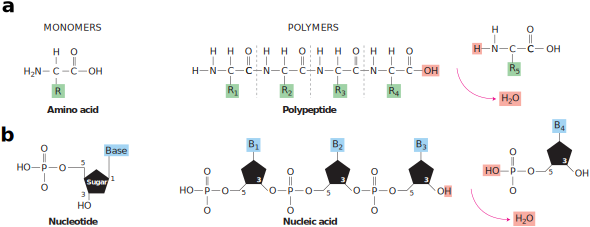
\includegraphics[width=0.99\textwidth]{lodish_56_dna_protein}
\caption[DNA and protein polymers]{\textbf{DNA and protein polymers.} (\textbf{a}) Representation of the monomer (amino acid) and polymer (peptidic chain) of the protein macromolecule. (\textbf{b}) Representation of the monomer (nucleotide) and polymer (nucleic acid) of the DNA macromolecule. In both polymers, new monomers can be added through a condensation reaction, which requires energy and liberates a water molecule (right side of the figure). \emph{Source: Lodish et al.}\cite{lodish2007} (modified to fit thesis format and/or clarify key points).}
\label{fig:lodish_dna_protein}
\end{figure}

% Global view of the function of proteins and DNA
The proteins assume many roles within (and outside of) the cell: catalysis of chemical reactions (enzymes), metabolite processing, cell signaling, regulation of the production of more proteins, structural function and others. Based on the protein's high frequency in metabolic activities, high number of different protein types and great variety of processes in which proteins are associated with, one might regard this polymer as having a central role in the maintenance of living organisms. On the other hand, the nucleic acids can be of two types: the deoxyribonucleic acid (DNA) and ribonucleic acid (RNA). The main function of the DNA is to store the hereditary information of the organism. It is based on such information that new proteins are generated by celullar processes. The RNA have many important functions which can be summarized as playing a fundamental role on the processes necessary for the manifestation of the information contained in the DNA.

% DNA structure
The DNA molecule is formed by a double helix of paired polymeric chains, each of which composed of the nucleotide types: adenine (A), cytosine (C), guanine (G) and thymine (T). Each nucleotide is composed by a sugar (deoxyribose), a phosphate group and a nitrogenous base (which determines the nucleotide type; see Figure~\ref{fig:lodish_dna_protein}). Within each DNA strand of the double helix, nucleotides are connected through phosphodiester bonds (strong covalent bonds). Between each DNA strand, nucleotides are paired and connected through hydrogen bonds (weaker than covalent bonds). Cytosines always pair with guanines and adenines always pair with thymines. Consequently, we call these base pairs complementary. Because nucleotides are paired between the double helix structure, is very common to refer to nucleotides as base pairs (bp). The Figure~\ref{fig:alberts_dna_structure} depicts a graphical representation of the DNA molecule.

% Figure - DNA structure
\begin{figure}[h!]
\centering
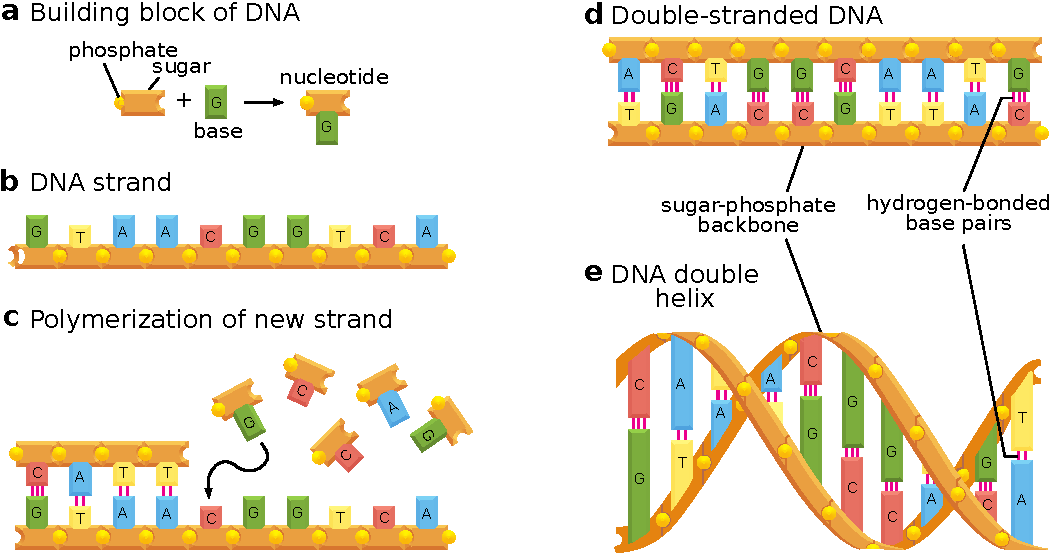
\includegraphics[width=0.99\textwidth]{alberts_37_dna_structure}
\caption[DNA structure]{\textbf{DNA structure.} (\textbf{a}) Representation of the DNA monomer (nucleotide) composed by a sugar, phosphate and a nitrogenous base. (\textbf{b}) Multiple nucleotides from all possible types that occurs in DNA (A, C, G and T), connected through phosphodiester bonds. This structure forms a single strand of DNA, which  in humans can be as long as \approxy$250,000,000$ nucleotides (human chromosome~1). (\textbf{c}) The DNA usually occurs as a double strand. The biological process of polymerization allows the addition of nucleotides to a single strand, forming the DNA double strand. Cytosines (C) always pair with guanines (G) connected through three hydrogen bonds (pink lines); and adenines (A) always pair with thymines (T) through two hydrogen bonds. (\textbf{d}) Linear scheme of the double DNA strands. (\textbf{e}) Double helix structure of the double-stranded DNA molecule. This is the general structure in which the DNA occurs in nature. \emph{Source: Alberts et al.}\cite{alberts2007} (modified to fit thesis format and/or clarify key points).}
\label{fig:alberts_dna_structure}
\end{figure}

% RNA structure
The RNA molecule differs from the DNA molecule because it contains another sugar type composing its nucleotides: the ribose. Since the ribose sugar provides greater stability to the RNA, it is generally found as a single strand. However, this single strand is able to hybridize (bind through hydrogen bonds to complementary nucleotides) with itself and fold, creating higher order structures. Also, the thymine nucleotide is replaced in the RNA structure by the uracil (U). RNA molecules perform many roles in the organism. Consequently, there is an extensive nomenclature for RNA molecules, based on their structure and function.

% Protein structure dictates function
Proteins are chemical compounds with high molecular weight formed by a variable-length chain of amino acids. Proteins consist in, approximately, $80\%$ of the dry weight of a cell. The amino acids that forms the proteins are composed of a central carbon atom which binds to a hydrogen, a carboxyl group, an amine group and a side chain (see Figure~\ref{fig:lodish_dna_protein}). The side chain may be of various types and dictates the type of the aminoacid. There are 20 amino acid types which are more common to be found at proteins. The specific order of each amino acid type in a protein determines its three-dimensional structure, given each amino acid's physicochemical properties. It is well-known that the protein structure is directly related to its function. The simple substitution of one amino acid in the proteic chain is sufficient to modify the protein three-dimensional conformation leading to a reduced functional capability or complete protein disfunction. The Figure~\ref{fig:villarreal_protein} shows the different levels of protein structural conformation.

% Figure - Protein structure
\begin{figure}[h!]
\centering
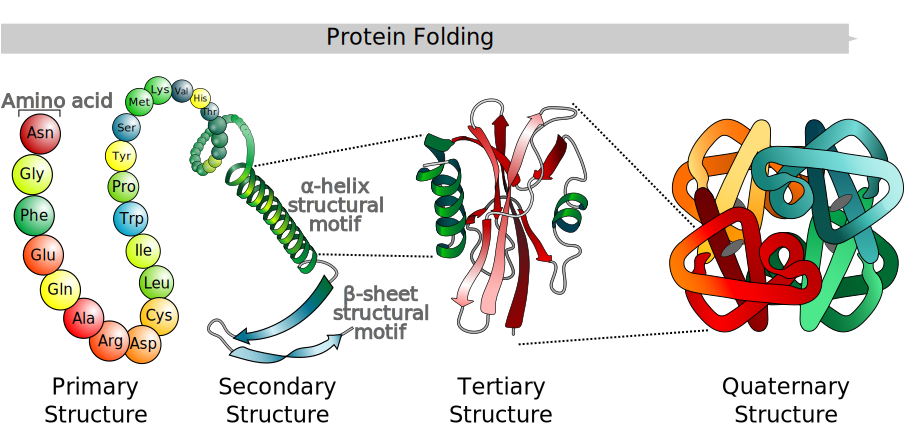
\includegraphics[width=0.50\textwidth]{villarreal_protein}
\caption[Protein structure]{\textbf{Protein structure.} Proteins are polymers formed by monomers termed amino acids. The chain of amino acids that forms a specific protein is the protein's primary structure. The protein secondary structures, such as $\alpha$-helixes or $\beta$-sheets, are formed through the natural folding of the amino acid chain given their physicochemical properties. The terciary structure are composed by a number of secondary structures forming a stable protein unit. Finally, the quaternary structure represents the aggregation of multiple protein units to form fully functional protein molecule complexes. \emph{Source: Mariana R. Villarreal} (modified to fit thesis format and/or clarify key points).}
\label{fig:villarreal_protein}
\end{figure}

% Central dogma introduction
The central dogma of molecular biology refers to the process in which proteins are created based on the information encoded in the cell's DNA. Only the key parts of this process, which aid in the understanding of this work, will be presented: (1) the transcription -- in which DNA information is converted into RNA molecules and (2) the translation -- in which the RNA information is converted into proteins.

% Transcription - introduction
The transcription is the central dogma's step responsible for generating an RNA molecule based on a specific portion of the DNA molecule. These specific portions are the so-called genes. Many proteins are required during the transcription step. Here we will focus on the RNA polymerase protein, which is involved in all three transcription steps: (1) the initiation (sometimes refered to as activation), (2) the elongation and (3) the termination.

% Transcription - process
During the iniciation phase, the RNA polymerase binds to a specific DNA region called promoter. After binding, the DNA double helix around the binding site uncoils, allowing that the RNA polymerase, which is bound to one of the DNA strands, continue the process. Then, the elongation phase begins, where the RNA polymerase starts to move through the DNA generating an RNA molecule. After each DNA nucleotide ``read'' by RNA polymerase, a new RNA nucleotide is added to the newly created RNA molecule, based on the affinity between nucleotides. While this process contnues through the extent of the gene, the RNA polymerase will keep uncoiling the DNA ``ahead'' and also re-hybridizing the DNA ``behind'' it. The DNA sequence ``ahead'' is termed ``downstream'' and the DNA sequence ``behind'' is termed ``upstream''. Finally, in the termination phase, the RNA polymerase destabilizes, detaches from the DNA and releases the new RNA molecule.

% Transcription - strands and order
It is important to mention that, although only one of the DNA strands is read during the transcription process, both strands contain information necessary to produce RNA. Another important issue is the orientation of these two DNA strands. Each strand has two extremities: one corresponding to a hydroxyl group attached to the $3^\prime$ carbon atom of the sugar; and the other corresponding to the phosphate group attached to the $5^\prime$ carbon atom of the sugar. For this reason, processes involving the sliding of proteins in DNA have two orientations: sense ($5^\prime \rightarrow 3^\prime$) and antisense ($3^\prime \rightarrow 5^\prime$). The different strands in the DNA helix are attached to each other in opposite (anti-parallel) orientations. The transcription always occurs in the sense orientation.

% RNA processing
After transcription, the RNA molecule goes through several editing steps, which change depending on the RNA type. The RNA that encodes information necessary to create a protein is called messenger RNA (mRNA). The mRNA will undergo several processes such as splicing, $5^\prime$-capping and $3^\prime$-polyadenylation. After that, the mRNA leaves the cell nucleus.

% Translation - process
The translation step consists in processing the mRNA in order to assemble a protein using aminoacids. The main structure associated to the translation is the ribosome, that is mainly located in the cell's cytoplasm and is composed of proteins and RNA. The translation initiates when the ribosome binds the mRNA. Each triplet of RNA's nucleotides (termed codon) is ``read'' by the ribosome, which will attach a specific amino acid to the protein being produced. Each one of the 20 basic amino acids corresponds to one or more of the 64 codons. There are specific codons to indicate the exact position in the RNA where the translation starts and ends.

% Translation - post-translational modifications
The final proteins created through the translation will conform according to the physicochemical properties of the amino acids influenced by the aqueous cytoplasmic environment. After assuming its final form, the protein is ready to perform its function. Some proteins might undergo the so-called post-translational modifications, such as the further addition of methyl groups in some amino acids. This fact will be further explored later in this chapter. The Figure~\ref{fig:lodish_central_dogma} exhibits a graphical representation of the central dogma's steps discussed here.

% Figure - Central dogma of molecular biology
\begin{figure}[h!]
\centering
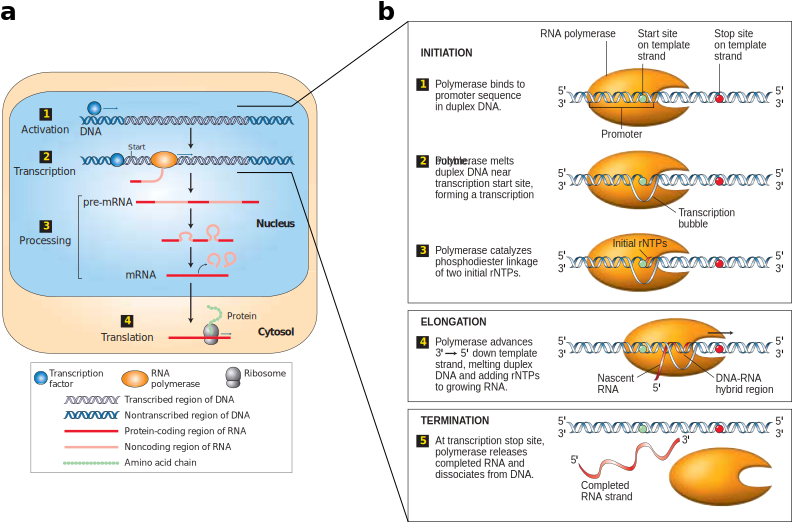
\includegraphics[width=0.99\textwidth]{lodish_30_central_dogma}
\caption[Central dogma of molecular biology]{\textbf{Central dogma of molecular biology.} (\textbf{a}) Depiction of the main steps of the central dogma of molecular biology necessary to create a protein molecule from the information encoded within the DNA molecule. Here we show the steps: (1) transcription initiation, (2) transcription elongation, (3) RNA processing and (4) translation. (\textbf{b}) In this work, we focus on the transcription. Thus, we show a graphical representation of the transcription steps discussed here. \emph{Source: Lodish et al.}\cite{lodish2007} (modified to fit thesis format and/or clarify key points).}
\label{fig:lodish_central_dogma}
\end{figure}

% Conclusion
This section provided a brief and simplified overview on the basic structures and processes necessary to the understanding of this work. The next section will further explore the initiation step of the transcription process, highlighting the known mechanisms that contributes for the spatial and temporal regulation of which genes are going to be transcribed, i.e. which genes are going to be expressed.

%%%%%%%%%%%%%%%%%%%%%%%%%%%%%%%%%%%%%%%%%%%%%%%%%%%%%%%%%%%%%%%%%%%%%
% Section: Eukaryotic Regulation
%%%%%%%%%%%%%%%%%%%%%%%%%%%%%%%%%%%%%%%%%%%%%%%%%%%%%%%%%%%%%%%%%%%%%
\subsection{Eukaryotic Regulation}
\label{sec:eukaryotic.regulation}

% Introduction - eukaryotes
Living organisms can be divided into two groups: (1) prokaryotes -- the organism's genetic material (i.e. the DNA) is located in the cell's cytoplasm and presents a circular structure and (2) eukaryotes -- the organism's cells have a nucleus which contains, among other structures, the DNA. Here, we will focus on eukaryotes. Most eukaryotes have more than one DNA molecule, which are termed chromosomes. The set of a cell's chromosomes is called genome. Furthermore, some organisms present more than one copy of a chromosome. The human genome -- which is the main focus of this work -- presents two copies of 22 different chromosomes (refered to based on a number between 1--22) and two extra chromosomes (termed X and Y), which determines the individual's biological gender. This adds up to a total of $46$ chromosomes and classify humans as diploid organisms (have two copies of each chromosome).

% Introduction - Trascriptional regulation
In the previous section, it was discussed the basic concepts with regard to the process in which proteins are created based on DNA. The transcription initiation was previously described as the step in which the RNA polymerase binds to the promoter region in order to start the process of gene expression. However, there are many factors that contribute to the expression of particular genes in particular types/stages/conditions of a cell. We call ``gene regulation'' the wide range of mechanisms that are used by cells to increase or decrease the production of specific gene products.

% Regulatory elements - introduction
Gene regulation happens in different stages of the central dogma: transcription initiation, transcription elongation, mRNA processing, mRNA transport, translation and others. However, most part of the regulatory events happens at the transcription initiation level. A major role of the regulation at this level is played by proteins termed \emph{regulatory elements}, which use their physicochemical properties to direct the intensity level in which gene products are created.

% Regulatory elements - cis and trans
The regulatory elements can act in \emph{cis} or in \emph{trans}. The \emph{cis}-acting regulatory regions are defined as the DNA regions in the vicinity of the gene they regulate, which can be bound by \emph{trans}-acting regulatory elements (mostly proteins, which can be encoded far from the gene it regulates or even in another chromosome). Hereafter, we will extrapolate the traditional nomenclature and call the \emph{trans}-acting regulatory elements as transcription factors (TFs) -- which traditionally only consist of a subset of \emph{trans}-acting regulatory elements -- and the smaller \emph{cis}-acting regulatory regions' units where TFs bind to as transcription factor binding sites (TFBSs). \emph{Cis}-acting regulatory regions -- composed of one or more TFBSs -- can be divided into two different types: (1) regions close ($< $\approxy$1,000$ bp, i.e. $1$ Kbp) to a gene (promoter region or proximal regulatory region) and (2) DNA regions far (up to \approxy$1,000,000$ bp, i.e. $1$ Mbp) from genes (distal regulatory region). Different TFs may bind to TFBSs to increase or decrease the expression of genes. The Figure~\ref{fig:alberts_gene_regulation} shows a graphical representation of the regulatory elements discussed here.

% Figure - Regulatory elements
\begin{figure}[h!]
\centering
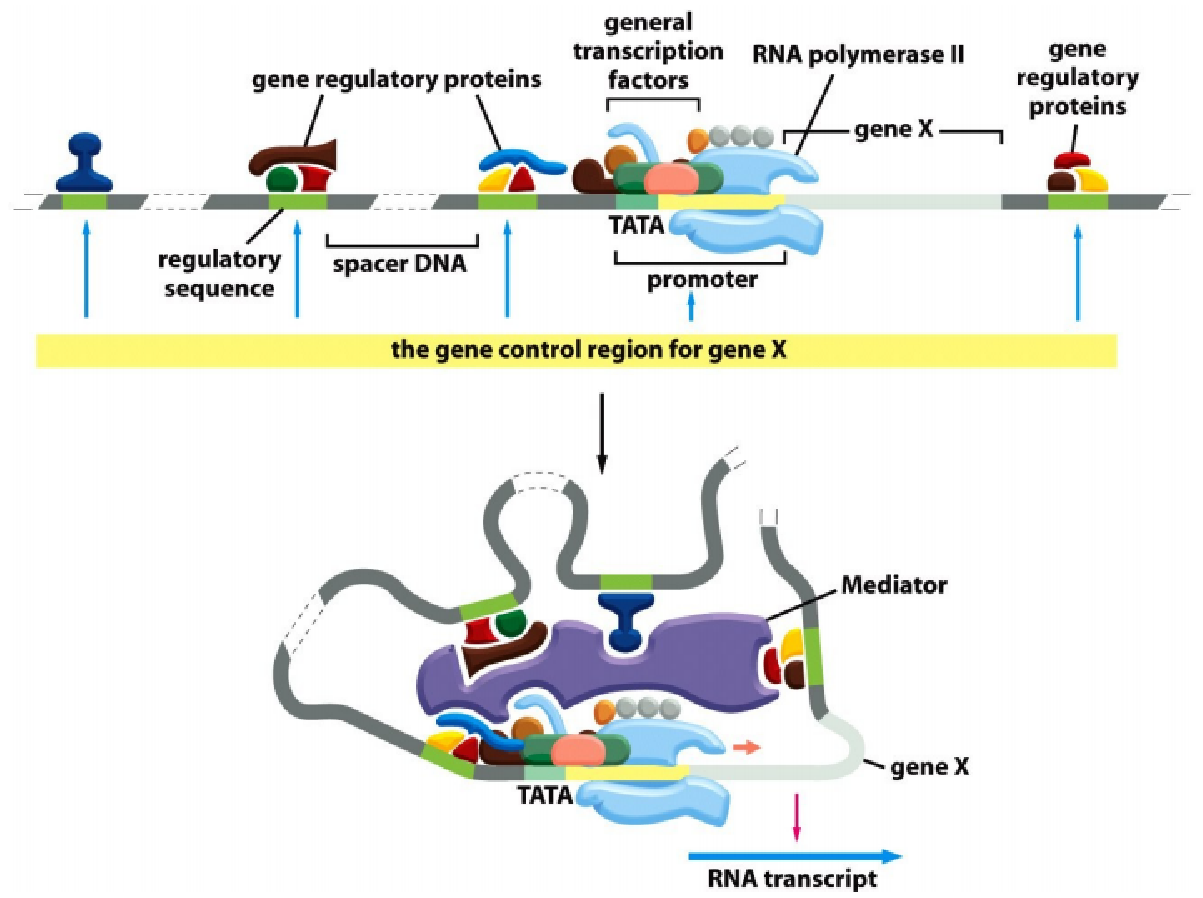
\includegraphics[width=0.80\textwidth]{alberts_475_gene_regulation}
\caption[Regulatory elements]{\textbf{Regulatory elements.} Schematic of a typical gene regulatory region with proximal and distal regulatory regions being bound by transcription factors. The promoter typically spans less than $1$ Kbp and is composed of: (1) a core promoter -- where the transcriptional machinery is being bound and (2) proximal promoter elements -- where transcription factors bind to increase/decrease gene expression. The distal (upstream/downstream) regulatory elements can be located up to $1$ Mbp pairs from the promoter. Among others, they include: (1) enhancers -- which transcription factors bind to increase gene expression; (2) silencers -- usually decreasing or completely silencing expression and (3) insulators -- which are boundary regions that are able to both repress enhancers and silencing mechanisms. These distal elements may contact the core promoter or proximal promoter through a mechanism that involves looping out the intervening DNA. \emph{Source: Alberts et al.}\cite{alberts2007} (modified to fit thesis format and/or clarify key points).}
\label{fig:alberts_gene_regulation}
\end{figure}

% Protein motifs
The transcription factors contain a specific part (formally called ``domains'') within their structure, termed active site, which enables them to bind to the DNA. Differently from what was thought when the first protein structures were characterized, there is a relatively short number of smaller structural variants (which compose the final protein structure) in comparison to the number of different protein types. Some of these structural variants, including the ones containing active sites, are repeated between different protein. These DNA-binding protein domains usually have affinities towards specific DNA sequences. These affinity sequences are termed ``motifs''. The Figure~\ref{fig:gusmao_binding_type} shows four DNA-binding protein domains and examples of proteins that contain such domains and their respective DNA binding affinity motifs. These affinities are graphically depicted using logo graphs, which will be introduced in Section~\ref{sec:motif.matching.method}.

% Figure - Different protein-DNA binding types
\begin{figure}[h!]
\centering
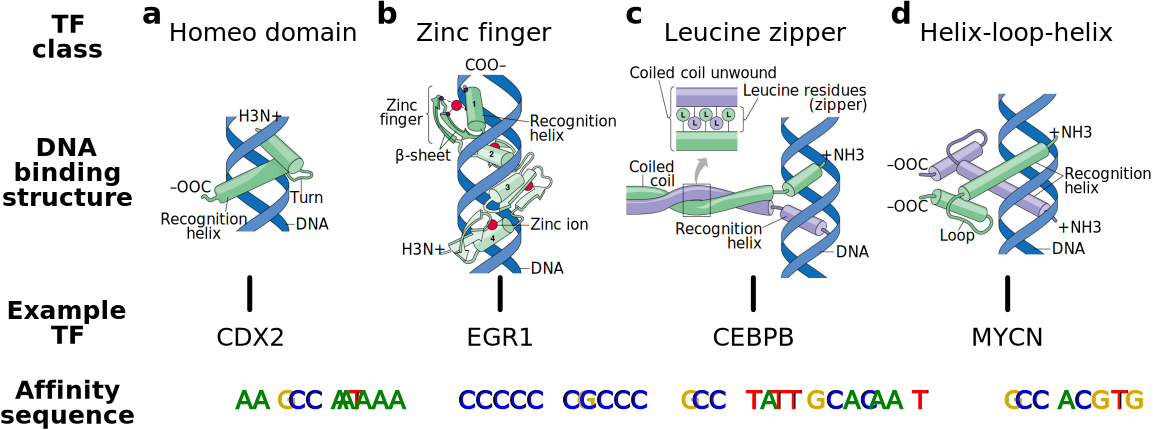
\includegraphics[width=0.99\textwidth]{gusmao_binding_type}
\caption[Different protein-DNA binding types]{\textbf{Different protein-DNA binding types.} We show graphical representations of different protein-DNA binding types (top) and examples of proteins with such binding domain type and their graphical DNA binding affinity information (bottom). These graphical binding affinity information is explained in Section~\ref{sec:motif.matching}. We show four DNA-binding types: (\textbf{a}) Homeo domain (also known as helix-turn-helix), (\textbf{b}) zinc finger, (\textbf{c}) leucine zipper and (\textbf{d}) helix-loop-helix. This motivates the idea that, although there are many DNA-binding proteins, they usually have a few DNA-binding domains. The protein DNA binding affinities are graphically depicted using logo graphs. Briefly, the larger the nucleotides are within each position of the binding site the more affinity such protein has to bind this nucleotide at that position.}
\label{fig:gusmao_binding_type}
\end{figure}

% Chromatin structure 1
Moreover, the regulatory elements here should also be discussed in the context of chromatin dynamics. The DNA is not isolated in the cell nucleus. Instead, it is found wrapped in proteic complexes which is associated to the compaction of the DNA within the cell nucleus and many regulatory events. Such DNA$+$protein structure is termed chromatin. The DNA is found wrapped in a set of eight proteins called histone complex, which are generally composed of four pairs of histones named H2A, H2B, H3 and H4. The unit composed by the DNA wrapped in approximately $1.65$ turns (\approxy$147$ bp) around the histone complex is called nucleosome. From this lower level structure (nucleosome) the chromatin structure can be compacted in many different levels. This compaction organization is depicted in Figure~\ref{fig:lodish_chromatin_structure}. Briefly, the chromatin can be found in a very condensed structure which does not allow transcription initiation (termed heterochromatin, or simply ``closed chromatin''); or in a decondensed form, allowing transcription initiation and gene expression (termed euchromatin, or simply ``open chromatin'').

% Figure - Chromatin conformation
\begin{figure}[h!]
\centering

\includegraphics[width=0.5\textwidth]{lodish_420_chromatin_structure}
\caption[Chromatin conformation]{\textbf{Chromatin conformation.} The nuclear DNA have many compaction levels. (\textbf{a}) It is depicted an entire chromosome in the cell's metaphase, which represents the higher degree of compaction the DNA can assume. (\textbf{b},\textbf{c}) The chromatin has many levels of compaction organized within the chromatin scaffold. (\textbf{d}) A lower ogranizational level -- termed $30$-nm fiber -- may assume many different configurations. (\textbf{e}) The DNA is wrapped around histone complexes. (\textbf{f}) Deepest organizational layer represented by the unwrapped DNA molecule. \emph{Source: Lodish et al.}\cite{lodish2007} (modified to fit thesis format and/or clarify key points).}
\label{fig:lodish_chromatin_structure}
\end{figure}

% Chromatin structure 2
Different parts of the genome can be open and closed at different times, allowing a specific set of genes to be expressed under different cell conditions. This is one of the main mechanisms in which we are able to observe such a high number of different cells, each of which expressing a different set of genes, given that they all share the same underlying genomic information encoded in the DNA. The chromatin can switch between closed and open states via two major chromatin remodelling mechanisms: (1) covalent post-translational histone modifications by specific enzymes such as histone acetyltransferases (HATs), deacetylases, methyltransferases and kinases and (2) ATP-dependent chromatin remodelling complexes which either move, eject or restructure nucleosomes. Here, we discuss the post-translational histone modifications.

% Histone modifications
The histone proteins n-terminal usually protrudes from the nucleosome and is termed histone tail. These histone tails can undergo post-translational chemical modifications at specific amino acids. These modifications include the methylation (addition of a methyl group), acetylation (addition of an acetyl group), phosphorylation (addition of a phosphoryl group), ubiquitylation (addition of a ubiquitin protein) and sumoylation (addition of SUMOs -- small ubiquitin-like modifiers). These modifications have a specific nomenclature dictated by: histone type, amino acid type, amino acid position within the histone tail and modification type. For instance, ``H3K4me1'' refers to the monomethylation (me1) of the fourth lysine (K4) of the tail of histone H3.

% Histone modification effects on chromatin
The histone modifications are directly associated to regulatory events since they change the accessibility of proteins to the DNA in the chromatin, enabling or disabling the binding of TFs. For instance, the HATs are able to transfer an acetyl group to certain amino groups of histone tail's lysine side chains. In doing so, they neutralize the lysine's positive charge and makes the interactions between histones and DNA weaker. Consequently, the DNA is more accessible for TF binding. The Figure~\ref{fig:lall_histone_modifications} displays the known effects of modifications in lysines in the tail of histone H3.

% Figure - Main histone modifications on lysines of histone H3
\begin{figure}[h!]
\centering
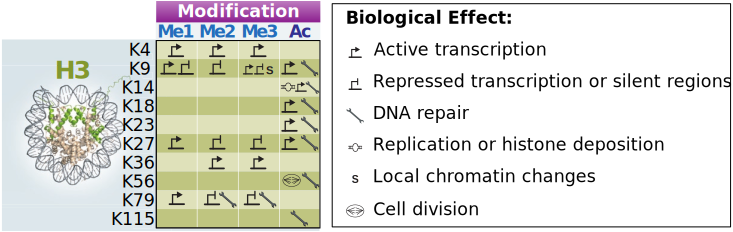
\includegraphics[width=0.7\textwidth]{lall_1111_histone_modifications}
\caption[Main histone modifications on lysines of histone H3]{\textbf{Main histone modifications on lysines of histone H3.} The tail of the histone H3 undergo post-translation modifications which are associated to chromatin remodelling. Different modifications at different locations of the H3's tail have contrasting effects such as transcription initiation or repression. \emph{Source: Lall et al.}\cite{lall2007} (modified to fit thesis format and/or clarify key points).}
\label{fig:lall_histone_modifications}
\end{figure}

%%%%%%%%%%%%%%%%%%%%%%%%%%%%%%%%%%%%%%%%%%%%%%%%%%%%%%%%%%%%%%%%%%%%%
% Section: Active Binding Site Detection
%%%%%%%%%%%%%%%%%%%%%%%%%%%%%%%%%%%%%%%%%%%%%%%%%%%%%%%%%%%%%%%%%%%%%
\section{Active Binding Site Detection}
\label{sec:active.binding.site.detection}

% Introduction to the problem
In Section~\ref{sec:eukaryotic.regulation}, we presented an overview of main features regarding eukaryotic gene regulation. The interplay between the regulatory elements presented vary depending on many circunstances. TFs are bound and release from TFBSs in a dynamic manner in conformity to the proper cellular development. Furthermore, this dynamic regulatory process colaborates with the orchestration of proper spatial and temporal expression of genes. In fact, complex regulatory networks govern multiple mechanisms which are crucial for the cell, such as: proliferation, development, signaling, differentiation, aging and apoptosis. Therefore, the identification of such regulatory elements is crucial to understand regulatory networks driving the aforementioned cellular processes and the onset of diseases which manifest due to regulatory network disruption. Given that, we can formally define the problem we are addressing in this work:

\vspace{0.5cm}
\noindent
\textbf{Active Binding Site Detection Problem:} \emph{For a given cell's genome, find all putative genomic regions (termed transcription factor binding sites; TFBSs) in which there are proteins (termed transcription factors; TFs) binding, playing a specific regulatory role in the gene expression of the cell.}
\vspace{0.45cm}

% Different approaches to handle the problem
The problem of active binding site detection has a few variants, depending mainly on the specific goals of research analyses. One the one hand, system-focused analyses require the identification of a few target binding sites. In this case, there is \emph{a priori} knowledge on the particular regulatory players involved at the particular mechanism being studied. On the other hand, system-exploratory analyses require a genome-wide map of all putative transcription factor binding sites that are being bound by proteins at a particular cell condition. In this case the researchers are interested in a genome-wide map of all putative active binding sites in order to perform various further inferences on the regulatory dynamics of the system under study.

% Importance of the problem - introduction
As previously mentioned, the identification of regulatory elements is a very important task, since they are the key players on most regulatory mechanisms. The subject under study can be a single cell's regulatory landscape or the mechanisms behind a system of two or more different cells. In the single cell's study we might be interested, among other, in the identification of regulatory elements associated with: (1) up/downrelgulation of a gene or group of genes; (2) group of genes interesting for a particular reason such as drug response; (3) viral infection and (4) cell signalling mechanisms. When studying more than one cells, on might be interested, for instance, in the detection of the regulatory elements related to: (1) cellular processes such as differentiation, apoptosis, aging and development; (2) cellular reponse to stimulus by studying the regulatory elements disposition before and after stimulus; (3) temporal cellular response to personalized therapies and (4) the mechanisms underlying diseases by comparing disease-affected cells with healthy cells.

% Importance of the problem - examples
There are a great number of studies that benefited from the proper identification of active binding sites. Recent studies, that uses technologies that will be described in Sections~{sec:ngs.methods} and~{sec:computational.footprinting.methods}, have particularly provided multiple insights on a different range of mechanisms such as cell differentiation and understanding the onset of diseases. For instance, studies were able to: (1) unravel cellular differentiation processes~\cite{lin2015,tsankov2015}; (2) unravel disease mechanisms~\cite{schaub2012,vernot2012,charos2012}; (3) perform gene expression prediction and high-order functional analyses~\cite{yip2012,whitfield2012,natarajan2012} and (4) understand other cellular regulatory elements such as long noncoding RNAs~\cite{tilgner2012,banfai2012}. In summary, the identification of active transcription factor binding sites is important because of its broad impact on many other cellular processes.

% Problem's issues
However, there are many issues that makes this a hard problem. First, the regulatory landscape is cell condition-specific, i.e. each cell undergoing a specific stage/process/condition/stimulus contains a different set of regions accessible by TFs. Also, there are over $1,500$ known TFs, each of which can bind to the DNA directly or by being recruited (such as co-activators). The possible combinatorial binding framework makes it very hard to unravel regulatory regions on a TF-wise approach. Furthermore, some TFs bind in a very dynamic manner, which makes hard to interpret a particular snapshot of the regulatory landscape captured at a specific moment of the cell's lifetime. Moreover, the DNA sequence affinity of TFs are usually very small, varying between 6--12 bp; and only a fraction of these nucleotides are well-conserved considering all binding sites.

% Small historical overview & overview to the next sections
In the following sections we will introduce the traditional computational method to predict transcription factor binding sites, termed motif matching, and its limitations (Section~\ref{sec:motif.matching}). Given this method's limitations, the state-of-the-art methods use novel experimental biological assays based on nex-generation sequencing techniques (Section~\ref{sec:ngs.methods}) coupled with computational frameworks. These recent methodologies to predict active binding sites, termed computational footprinting methods (Section~\ref{sec:computational.footprinting.methods}) are the subject of study of this work. We will explore how these methods work and provide a comprehensive literature review. Finally, we will describe the current challenges and problems not addressed by these methods and discuss our approach to address the problem of active transcription factor binding site prediction.

%%%%%%%%%%%%%%%%%%%%%%%%%%%%%%%%%%%%%%%%%%%%%%%%%%%%%%%%%%%%%%%%%%%%%
% Section: Motif Matching
%%%%%%%%%%%%%%%%%%%%%%%%%%%%%%%%%%%%%%%%%%%%%%%%%%%%%%%%%%%%%%%%%%%%%
\section{Motif Matching}
\label{sec:motif.matching}

% Introduction
With the increasing demand for methods that are able to analyze the whole genome, some computational approaches were developed in order to aid the genome-wide search of transcription factor binding sites. In this section the motif matching method will be described (Section~\ref{sec:motif.matching.method}). This method is based on a few preliminary experimental biological assays to determine the DNA sequence binding affinity (termed motif) that each protein has in order to create mathematical models that can be used to scan the genome for these binding affinity pattens. The particular motif matching variant shown here is based on Wasserman et al.~\cite{wasserman2004}. However, this approach has many limitations (Section~\ref{sec:motif.matching.limitations}). The main one is that it is not able to recover active sites, since it uses only the DNA sequence of a particular organism, ignoring the chromatin dynamics environment.

%%%%%%%%%%%%%%%%%%%%%%%%%%%%%%%%%%%%%%%%%%%%%%%%%%%%%%%%%%%%%%%%%%%%%
% Section: Motif Matching Method
%%%%%%%%%%%%%%%%%%%%%%%%%%%%%%%%%%%%%%%%%%%%%%%%%%%%%%%%%%%%%%%%%%%%%
\subsection{Motif Matching Method}
\label{sec:motif.matching.method}

% PFMs
Low-throughput biological assays such as chromatin immunoprecipitation (ChIP) are able to retrieve DNA sequences bound by a specific target protein in short genomic regions. Before the motif match procedure, we need to generate the mathematical representation of the underlying DNA sequences in which the target protein has binding affinity. To create such structure, first a multiple alignment algorithm is applied to the DNA sequences which are known to bind the target protein, i.e. that were obtained using an experimental biological technique. After that, conserved positions within this multiple alignment are determined and a specific window, that varies from $5$--$25$ bp is estimated to be the start and end position of the binding affinity representation. At this point, a matrix termed position frequency matrix (PFM) $\mathbf{X}^{4 \times N}$ is created in the following way: each matrix row $i \in D\}$ with $D = \{A,C,G,T\}$, correspond to each one of the possible four DNA nucleotides; and the each matrix column $ j \in \{1, ..., N\} $ correspond to a position within the motif in the multiple aligned DNA sequences. Consequently, $N$ represents the total length of the motif. Each entry $x_{ij}$ of the PFM corresponds to the number of nucleotides of type $ i $ in position $ j $ of the DNA framents' multiple alignment.

% PWMs
From PFMs, it is common to create normalized logarithmic representations termed position weight matrices (PWMs) $\mathbf{W}^{4 \times N}$. The most common method to create PWMs consists on the calculation of the corrected probability $ p_{ij} $ of finding the nucleotide $ i $ in the position $ j $, which is given by
\begin{equation}
  \label{eq:pwm1}
  p_{ij} = \frac{ f_{ij} + s(i) }{ N + {\sum\limits _{i^\prime \in D}{ \hspace{-0.0cm} s(i^\prime)}} }, 
\end{equation}
where $ f_{ij} $ is the frequency of base $ i $ at position $ j $ and $ s(i) $ is a pseudocount function. Pseudocounts are small values used to avoid null probabilities. After the evaluation of the corrected probabilities, the entries $ w_{ij} $ of the PWM can be calculated as
\begin{equation}
  \label{eq:pwm2}
  w_{ij} = \log_2 \frac{ p_{ij} }{ b(i) }, 
\end{equation}
where $ b(i) $ is the genomic frequency of nucleotide $ i $ in the genome. The background correction function $b(\cdot)$ is used to correct the PWM for biases regarding the genomic imbalance between the frequencies of the nucleotides.

% Information content
We are able to assess the information content $ \mathbf{l} = \langle{l}_{1}, ..., {l}_{N}\rangle $ of each position $ j $ of the PWM $ \mathbf{W} $ by applying
\begin{equation}
  \label{eq:pwm.ic}
  {l}_{j} = 2 + \sum\limits _{i \in D} p_{ij} \log_{2} p_{ij},
\end{equation}
where the number $2$ is obtained from the total possible information content of the $4$-character alphabet $D$, i.e. $\log_{2}4 = 2$. Based on the total information content for every position of the PWM, we are able to create graphical representations of the binding affinity -- termed logo graphs -- by multiplying the corrected probability of a certain nucleotide $i$ at a certain position of the PWM $j$ by the total information content at that position (${l}_{j}$). A summary of the PWM creation and score calculation can be seen in Figure~\ref{fig:wasserman_pwm}.

% Figure - Position weight matrices (PWMs)
\begin{figure}[h!]
\centering
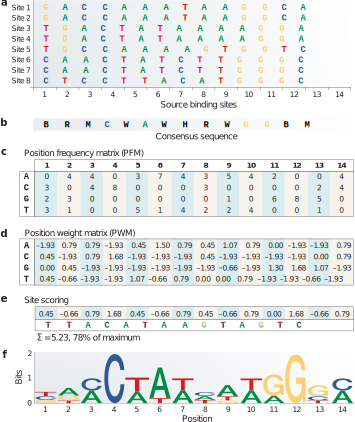
\includegraphics[width=0.65\textwidth]{wasserman_6_pwm}
\caption[Position weight matrices (PWMs)]{\textbf{Position weight matrices (PWMs).}The first step towards building models for predicting transcription factor (TF) binding sites involves data collection. To illustrate the process, we use the transcription factor MEF2 as an example. (\textbf{a}) A set of experimentally validated MEF2-binding sites was collected from the literature and aligned. The sequence variability of the collection of binding sites strongly affects the downstream models for predicting additional sites. Note the diversity between the sites; for instance, only $50\%$ of the nucleotides are identical between sites one and eight. (\textbf{b}) Here we show, for illustrative purposes, a consensus sequence model, which is defined by selecting a degeneracy nucleotide symbol for each position (column) in the alignment. For instance, the symbol ``B'' means preference for either nucleotides C, G or T. (\textbf{c}) To more accurately reflect the characteristics at each position, a matrix that contains the number of observed nucleotides at each position is created. For instance, the first column in the alignment consists of no As, three Cs, two Gs and three Ts, therefore resulting in the corresponding first matrix column $\langle 0, 3, 2, 3 \rangle$. (\textbf{d}) The frequency matrix is usually converted to a position weight matrix (PWM) using a the procedure described by Equations~\ref{eq:pwm1},~\ref{eq:pwm2}. (\textbf{e}) Using a matrix model, a quantitative score for any DNA sequence can be generated by summing the values that correspond to the observed nucleotide at each position. This procedure can be repeated for all contiguous sequences in the genome, which consist on the motif matching method, formally described by Equations~\ref{eq:motif.match}--\ref{eq:pwm.cutoff2}. (\textbf{f}) The specificity in each column of the alignment can be measured in terms of information content. A sequence logo scales each nucleotide by the total bits of information multiplied by the relative occurrence of the nucleotide at the position (see Equation~\ref{eq:pwm.ic}). Sequence logos enable fast and intuitive visual assessment of pattern characteristics. \emph{Source: Wasserman et al.}\cite{wasserman2004} (modified to fit thesis format and/or clarify key points).}
\label{fig:wasserman_pwm}
\end{figure}

% Motif matching
From a PWM it is possible to evaluate the probability of the particular TF, in which the PWM was created, of binding in the genome. We call this procedure motif matching. For each sequence of nucleotides of length $ N $, a bit-score can be evaluated. There are also many strategies to perform this calculation. The simples one is the summation of all the entries in $ w_{ij} $ matching the nucleotide sequence of length $ N $. More formally, given a sequence of characters $\mathbf{g}$ representing the genome, where $\mathbf{g} = \langle{g}_{1}, ..., {g}_{L}\rangle \forall {g}_{i} \in D$. We are able to define a vector of bit-scores $\mathbf{y} = \langle{y}_{1}, ..., {y}_{L-N}\rangle$ as
\begin{equation}
  \label{eq:motif.match}
  {y}_{i} = \sum_{j=1}^{N} \sum_{k \in D} {\mathbf{1}}(k={g}_{i}){w}_{kj},
\end{equation}
where ${\mathbf{1}}(\cdot)$ is an indicator function. 

% Motif match cutoff threshold
A genome-wide application of a PWM creates bit-scores for every possible contiguous nucleotide sequence of length $ N $ within the genome. Then, several statistical techniques can be used to determine a cutoff threshold to accept particular sequences as being bound by the protein, given the PWM. A well-known statistical procedure is to evaluate a bit-score cutoff that corresponds to the false positive rate (FPR) of the distribution of the bit-scores from all possible $N$-mers. More formally, let $C = \{\mathbf{{c}^{1}}, ..., \mathbf{{c}^{4^N}}\}$ be the set of all $N$-mers constructed by picking $ N $ elements from the set $ D $ with order and repetition, where each $N$-mer $\mathbf{{c}^{i}} = \langle{c}^{i}_{1}, ..., {c}^{i}_{N}\rangle$. Therefore, we are able to evaluate the set $ B = \{ {b}_{1}, ..., {b}_{4^N} \} $ of all the possible bit-scores for the PWM $\mathbf{W}$ as
\begin{equation}
  \label{eq:pwm.cutoff1}
  {b}_{i} = \sum_{j=1}^{N} \sum_{k \in D} {\mathbf{1}}(k={c}^{i}_{j}){w}_{kj}.
\end{equation}

Then, it is easy to find the FDR threshold by finding the $p$-value that corresponds to the distribution of $ B $ fitted to a certain distribution, say normal
\begin{equation}
  \label{eq:pwm.cutoff2}
  B \sim \mathcal{N}({\mu},{\sigma}^{2}).
\end{equation}
In this work, we will call the motif match putative binding site predictions as motif-predicted binding sites (MPBSs).

%%%%%%%%%%%%%%%%%%%%%%%%%%%%%%%%%%%%%%%%%%%%%%%%%%%%%%%%%%%%%%%%%%%%%
% Section: Motif Matching Limitations
%%%%%%%%%%%%%%%%%%%%%%%%%%%%%%%%%%%%%%%%%%%%%%%%%%%%%%%%%%%%%%%%%%%%%
\subsection{Motif Matching Limitations}
\label{sec:motif.matching.limitations}

% Motif matching disadvantages - minor
Some versions of the motif matching method have very reasonable accuracy rates and the motif matching's computational complexity makes it much easier to apply than the highly-technical and time-consuming biological assays. However, this technique has many intrinsic disadvantages. First, PWMs are generally small (usually between $5$--$20$ bp) and degenerate (only a fraction of the motif is highly conserved). Consequently, establishing a threshold that does not bias the analysis towards very high or very small number of MPBSs is very hard. Second, although there are currently some well-established PFM repositories, PFMs are not available for all TFs. One of the main reasons for that is the bottleneck generated by the requirement of \emph{a priori} biological assays. Third, the quality of such \emph{a priori} biological assays has a direct impact on the performance of PFM models. Fourth, some transcription factors bind in the genome through other co-factors. Therefore, the creation of PWMs for these factors is very hard since these co-binding partners might change under different circumstances. Fifth, some transcription factors do not bind directly on the DNA, they only have domains that interact with other proteins binding on the DNA. Thus, it is impossible to create a sequence-based affinity model for such transcription factors. Sixth, the accuracy of this method highly depends on the algorithms for PWM estimation, the motif matching algorithm and the statistical approach used to determine the bitscore cutoff threshold. Such variables tend to be highly sensitive between different organisms and TFs, making the experiment design complex.

% Motif matching disadvantages - major
However, the main disadvantage of such method is the fact that it is unable to identify active binding sites, i.e. binding sites that are actually being bound by proteins at a specific cellular condition. This happens because the motif match method relies only on the DNA sequence affinity of proteins. However, the DNA sequence is the same within cells for a particular organism; independent of cellular condition, life stage, stimuli response, and others. What changes between the cells of an organism is the chromatin structure.

% Chromatin structure provides cell-specificity
Different parts of the genome can be open and closed at different times, allowing a specific set of genes to be expressed under different cell conditions. This is one of the main mechanisms in which we are able to observe such a high number of different cells, each of which expressing a different set of genes, given that they all share the same underlying genomic information encoded in the DNA. The Figure~\ref{fig:lodish_open_closed_chromatin} shows a graphical example of two cells at different stages of commitment. Although the genomic region (locus) depicted is the same for these two cells, one present a closed chromatin structure, while the other present an open chromatin structure. The closed chromatin observed for the long-term hepatopoietic stem cell (Figure~\ref{fig:lodish_open_closed_chromatin}a) does not allow the gene ATF3 to be transcribed, while the open chromatin structure present in the monocyte cell (Figure~\ref{fig:lodish_open_closed_chromatin}b) does allow the expression of ATF3 gene, since the transcription factors and transcription machinery are able to access that region and start the transcription process.

% Figure - Open versus closed chromatin
\begin{figure}[h!]
\centering
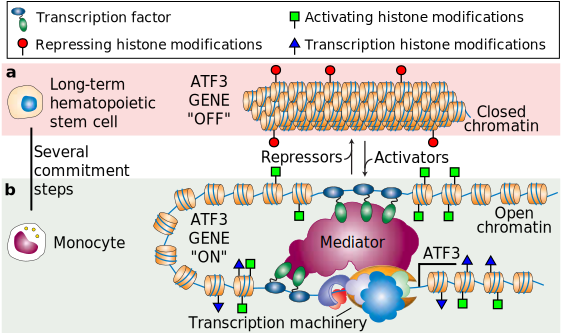
\includegraphics[width=0.8\textwidth]{lodish_461_open_closed_chromatin}
\caption[Open \emph{versus} closed chromatin]{\textbf{Open \emph{versus} closed chromatin.} Transription factor binding sites are cell-condition specific. This means that the same genomic locus might be accessible in a particular cell condition and not accessible in other condition. Such chromatin dynamics, which are modulated by genetic and epigenetic factors such as histone modifications, are responsible for the specialization of cells in performing the particular tasks required by the tissues they are located. This figure shows a graphical example of a locus (ATF3 gene) which is (\textbf{a}) closed in long-term hematopoietic stem cells (\textbf{b}) open in monocytes. Monocytes are a product of multiple specialization steps in hematopoietic stem cells. In this figure we show histone modifications which marks open/closed chromatin and proximal/distal regulatory regions. \emph{Source: Lodish et al.}\cite{lodish2007} (modified to fit thesis format and/or clarify key points).}
\label{fig:lodish_open_closed_chromatin}
\end{figure}

% Impact of chromatin structure on motif match
Therefore, the motif match method is not able to capture the active (cell-specific) binding sites. This is usually expressed practically on a very high number of false positive predictions, which represent the transcription factor binding sites which are not being accessed in a particular cellular condition. Consequently, in order to remove this very high number of false positive predictions, current methods rely on the use of biological assays that provide such cell-specificity. These assays are able to narrow the search space to the regions of open chromatin depicted in Figure~\ref{fig:lodish_open_closed_chromatin} and will be discussed in the following section.

%%%%%%%%%%%%%%%%%%%%%%%%%%%%%%%%%%%%%%%%%%%%%%%%%%%%%%%%%%%%%%%%%%%%%
% Section: Next-Generation Sequencing Methods
%%%%%%%%%%%%%%%%%%%%%%%%%%%%%%%%%%%%%%%%%%%%%%%%%%%%%%%%%%%%%%%%%%%%%
\section{Next-Generation Sequencing Methods}
\label{sec:ngs.methods}

% Introduction on NGS
Recently, novel DNA sequencing platforms have enabled the sequencing of a large number of DNA fragments at a given assay with a significant decrease in cost and complexity, when compared to traditional low-throughput methods~\cite{hayden2014}. We refer to these novel sequencing platforms as next-generation sequencing (NGS)~\cite{shendure2008}. The first of the NGS technologies -- massively parallel signature sequencing (or MPSS) -- was developed in the ${90}^{s}$ at Lynx Therapeutics. MPSS was a bead-based method that used a complex approach of adapter ligation followed by adapter decoding, reading the sequence in increments of four nucleotides~\cite{tucker2009}. Since then, NGS technologies are constantly improving. Some examples of modern techniques are: (1) Pyrosequencing (454)~\cite{margulies2005}, (2) Sequencing by synthesis (Illumina)~\cite{bentley2008}, (3) Sequencing by ligation (SOLiD sequencing)~\cite{valouev2008}, (4) Single-molecule real-time sequencing (Pacific Biosciences)~\cite{eid2009} and (5) Ion semiconductor (Ion Torrent sequencing)~\cite{pennisi2010}. A complete discussion on NGS can be found at Rusk et al.~\cite{rusk2010}.

% Adapt old techniques
The emergence of NGS and its constant technological improvements, have enabled traditional biological assays to detect active transcription factor binding sites, such as DNase I footprinting and chromatin immunoprecipitation (ChIP) to be revisited. On revisiting such methods, their protocols could be adapted in order to fit the NGS technologies, which enables these traditional low-throughput assays to be performed in a genome-wide manner.

% DNase-seq and ChIP-seq
In this section we will describe the following techniques: (1) DNase I footprinting followed by NGS (DNase-seq) -- which is an adaptation of the traditional low-thoughput DNase I footprinting and (2) Chromatin immunoprecipitation followed by NGS (ChIP-seq) -- which is an adaptation of the traditional low-throughput ChIP technique. Both techniques are now able to be performed in a genome-wide manner.

%%%%%%%%%%%%%%%%%%%%%%%%%%%%%%%%%%%%%%%%%%%%%%%%%%%%%%%%%%%%%%%%%%%%%
% Subsection: DNase-seq
%%%%%%%%%%%%%%%%%%%%%%%%%%%%%%%%%%%%%%%%%%%%%%%%%%%%%%%%%%%%%%%%%%%%%
\subsection{DNase-seq}
\label{sec:dnase.seq}

% DNase-seq intro
The DNase-seq technique~\cite{crawford2004,sabo2004a} consists in the observation of the DNA digestion by a certain cleavage agent able to break the phosphodiester bonds of the DNA molecule. The cleavage agent used in this method is the endonuclease deoxyribonuclease I (DNase I). This enzyme is capable of binding at the DNA double helix's minor groove and break the phosphodiester bond. This enzyme is of particular interest to this experiment design because of its great size, which makes it sensitive to proteins bound on DNA. Also, the action of DNase I can be easily controlled with ethylenediaminetetraacetic acid (EDTA).

% DNase-seq process - dnase I digestion
The DNase-seq method needs a high number of cells to start the protocol. This number varies between $10^{6}$--$10^{7}$. Furthermore, the protocol needs, on average, three to four days for preparation~\cite{buenrostro2013}. The protocol starts by isolating the cells' nuclei and breaking them in order to access the genomic material. The isolated (washed) genomic material will be treated with optimal concentrations of DNase~I, which will cleave the chromatin at random accessible positions. These accessible positions are the chromatin regions in which the DNA is open (see Figure~\ref{fig:lodish_open_closed_chromatin}) and not being bound by proteins such as transcription factors.

% DNase-seq process - fragment size selection - single hit
At this point -- after DNase I digestion -- there are two different protocols that will be explored here. In the first protocol, termed single-hit DNase-seq~\cite{crawford2004}, digested fragments are going to be filtered by size. Fragments in the order of $1,000$ Kbp are selected, representing the extremities of open chromatin regions, which include the upstream/downstream closed chromatin regions. After selecting for these longer fragments, biotinylated linkers will be add to the digested fragments and the solution will be treated with the type II restriction enzyme MmeI. The MmeI protein is able to recognize the added linker and cleave the DNA fragment at about $20$ bp upstram/downstrem from the DNase~I cleavage event. At this stage we have a short DNA fragment of $20$ bp plus the first linker. Then, a second linker is added to the site where the MmeI enzyme cleaved the DNA fragment and this ditagged $20$ bp DNA fragment is amplified through PCR.

% DNase-seq process - fragment size selection - double hit
On the other hand, in the second protocol, termed double-hit DNase-seq~\cite{sabo2004a}, the fragment size selection will be performed in the opposite fashion. In this case, only smaller fragments, in the order of $50$--$300$ bp are selected. It was recently observed that smaller fragment sizes ($50$--$100$) lead to optimal results~\cite{he2014}. These fragments represent whole DNA fragments contained within open chromatin regions and do not need further MmeI processing since they are already small enough to be treated with the necessary linkers and amplified through PCR.

% DNase-seq process - library preparation and sequencing
In both protocols, after PCR and DNA sequence library preparation, the resulting DNA fragments -- which are going to be referred in this work as ``reads'' -- are sequenced through NGS techniques. These steps require some additional experimental sample treatment which are out of scope of this simplified discussion.

% DNase-seq process - mapping back to genome (introduce idea of genomic signal)
After the sequencing, the resulting DNA sequences (reads) can be mapped back into the reference genome. This can be performed using a computational alignment tool such as Bowtie~2~\cite{langmead2012} or the Burrows-Wheeler Aligner (BWA)~\cite{li2009b}. These tools will map these short reads in the genome in a fast and accurate way. Afterwards, we are able to create a genomic signal by counting the number of overlapping reads at every genomic position. In the DNase-seq case, we only count the $5^{\prime}$ position of the reads, since that is the position in which the DNase~I enzyme has cleaved the DNA and indicates an open chromatin region. The Figure~\ref{fig:gusmao_dnaseseq} summarizes both protocols discussed here in a simplified flowchart. Details and mathematical formalization of the genomic signal generation are going to be performed in Section~\ref{sec:genomic.signal}.

% DNase-seq conclusion
The resulting genomic signal will represent a base-pair resolution map of the open chromatin positions within the whole genome. Each region enriched with DNase-seq reads -- termed DNase I hypersensitivity sites (DHSs) -- are composed of several DNase-seq signal peaks. The depletions within two of these base-pair resolution peaks are indicative of a region which the DNase~I enzyme could not access because there was probably a protein binding in that region. These depleteions between two peaks are called footprints and the identification of these regions gives us a genome-wide map of putative active transcription factor binding sites.

% Figure - DNase I sequencing experimental technique (DNase-seq)
\begin{figure}[h!]
\centering
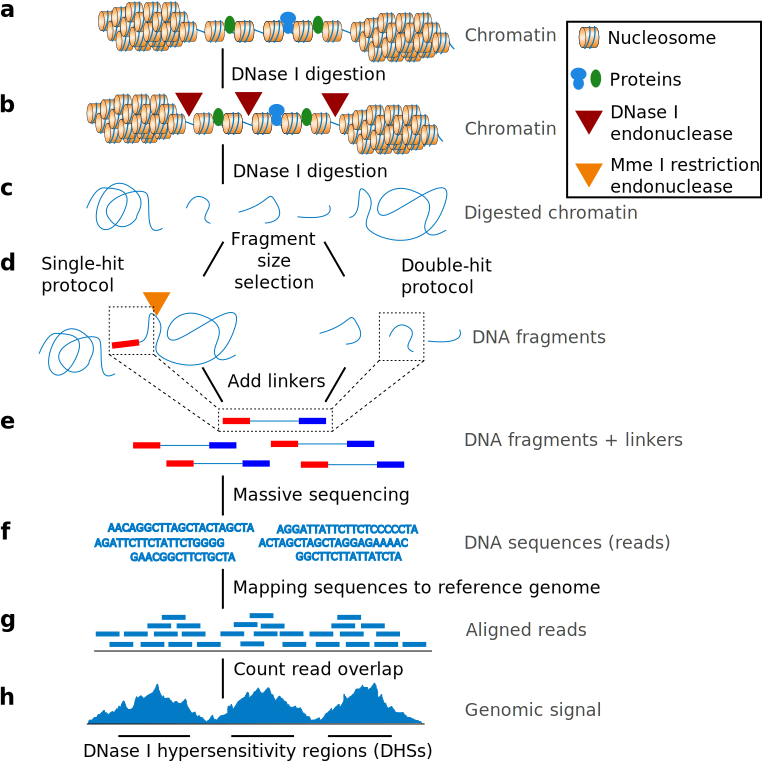
\includegraphics[width=0.85\textwidth]{gusmao_dnaseseq}
\caption[DNase I sequencing experimental technique (DNase-seq)]{\textbf{DNase I sequencing experimental technique (DNase-seq).} (\textbf{a}) The protocol starts by fetching the chromatin from multiple cells. (\textbf{b}) The chromatin is treated with optimal levels of DNase I enzyme, which will cleave the chromatin in accessible sites. These accessible sites are the ones in which the chromatin is open and is not being bound by TFs. (\textbf{c}) After the DNase I digestion we have multiple fragments of sheared chromatin (for simplicity, nucleosomes and proteins are not shown). (\textbf{d}) The chromatin fragments are selected for size, which distingishes the two protocol variants: (1) single-hit -- which selects the longer sequences representing the edges of an open chromatin region and (2) double-hit -- which selects the short sequences within open chromatin regions. In the single-hit variant, linkers (red box) are added to the chromatin fragments' extremities, which are recognized by the MmeI enzyme. Such enzyme will perform a cleavage event at about $20$ bp from the recognized linker sequence. Double-hit fragments are already small enough to be directly treated with linkers. (\textbf{e}) Linkers are added and a sequence DNA fragment library is prepared. (\textbf{f}) The DNA fragments are sequenced using NGS-based techniques. (\textbf{g}) The aligned DNA sequences are mapped back into the reference genome. (\textbf{h}) A signal can be generated by counting the overlap of the mapped DNA sequences. Regions with high concentration of DNase-seq reads are termed DNase I hypersensitivity sites (DHSs). Each of these regions are characterized by a number of peaks (not shown in this figure) which represent transcription factor footprints (see Figure~\ref{fig:gusmao_grammar_tfbs}).}
\label{fig:gusmao_dnaseseq}
\end{figure}

%%%%%%%%%%%%%%%%%%%%%%%%%%%%%%%%%%%%%%%%%%%%%%%%%%%%%%%%%%%%%%%%%%%%%
% Subsection: ChIP-seq
%%%%%%%%%%%%%%%%%%%%%%%%%%%%%%%%%%%%%%%%%%%%%%%%%%%%%%%%%%%%%%%%%%%%%
\subsection{ChIP-seq}
\label{sec:chip.seq}

% ChIP-seq introduction
The ChIP-seq technique~\cite{johnson2007} consists on the immunoprecipitation of target DNA-bound proteins and further sequencing of the DNA fragments fetched using NGS techniques. These target proteins can be, for instance, transcription factors or histones with a particular post-translational modification.

% ChIP-seq process - recapitulate similar steps of ChIP
The ChIP-seq protocol starts by isolating the cells' nuclei and breaking them in order to access the genomic material. The isolated (washed) genomic material is cross-linked in order to preserve all protein-DNA binding events. Next, the crosslinked chromatin is sheared into approximately $200$ bp DNA fragments with any massive shearing procedure (sonication, ultraviolet radiation or endonucleases). Afterwards, the chromatin lysate is treated with an antibody that targets a particular protein of interest. The solution is then immunoprecipitated. In this procedure, we fetch only the sheared chromatin fragments that contains the protein of interest. The immunoprecipitated solution is separated and washed in order to keep only the DNA fragments. Then, similarly to the DNase-seq protocol, these fragments are treated with linkers and a DNA fragment library is prepared and amplified in order to be sequenced by NGS techniques.

% ChIP-seq process - genomic signal
As described in the Section~\ref{sec:dnase.seq}, sequenced DNA fragments (reads) can be mapped back into the reference genome and a genomic signal can be created. The difference here is that the ChIP-seq signal has a lower resolution than the DNase-seq signal. This happens because, before mapping back the DNA sequences into the genome, we extend these small reads to the total average original immunoprecipitated fragments' length, which is \approxy$200$ bp. The extension is performed because the target protein can be located virtually at any position of the immunoprecipitated fragment. Then, unlike the DNase-seq protocol in which only one position (where the DNase I enzyme has nicked the DNA) is counted to generate the signal, the ChIP-seq signal is generated by counting the overlap of the whole extended fragment. In practise, ChIP-seq generates more smoothed signals than DNase-seq. The Figure~\ref{fig:gusmao_chipseq} summarizes the ChIP-seq technique in a simplified flowchart.

% Figure - ChIP sequencing experimental technique (ChIP-seq)
\begin{figure}[h!]
\centering
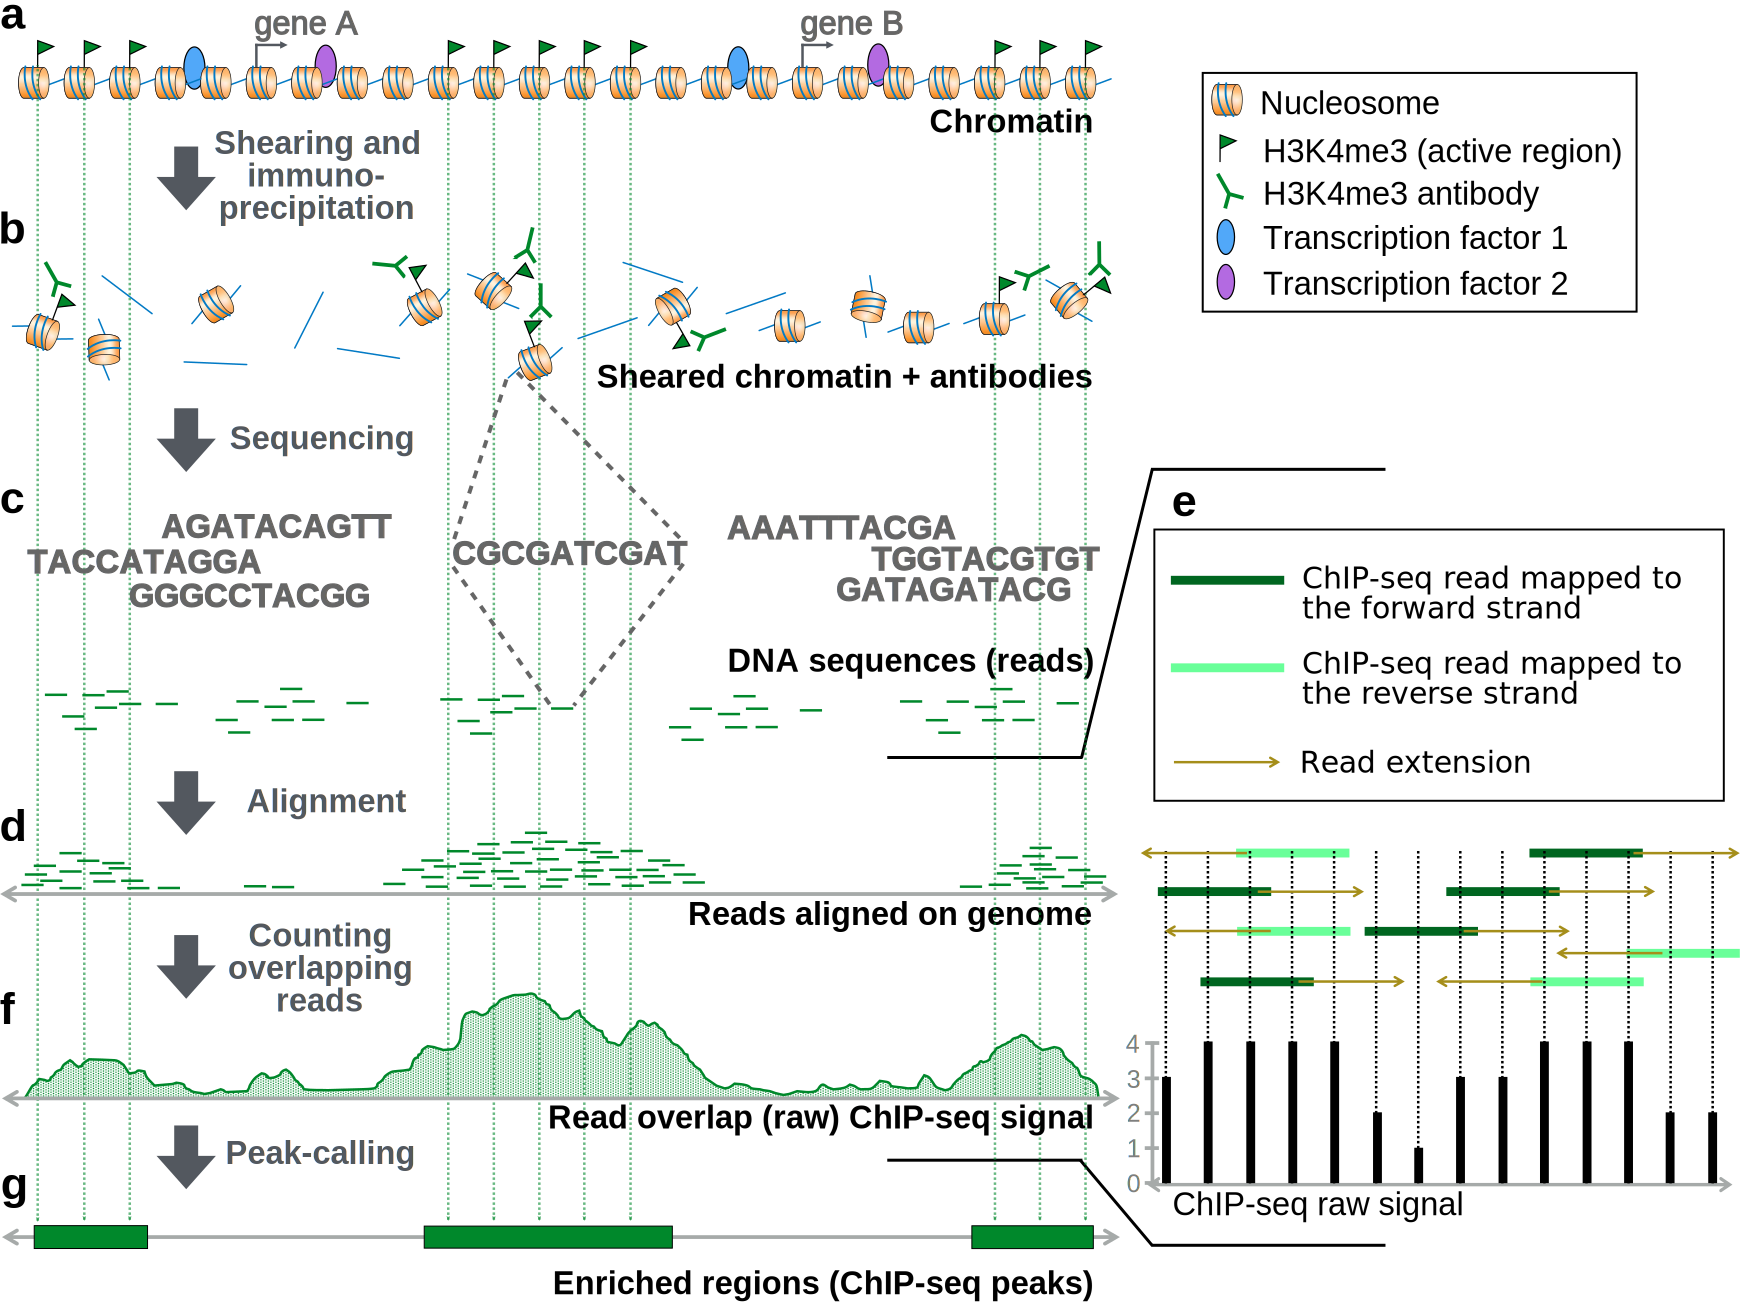
\includegraphics[width=0.85\textwidth]{gusmao_chipseq}
\caption[ChIP sequencing experimental technique (ChIP-seq)]{\textbf{ChIP sequencing experimental technique (ChIP-seq).} (\textbf{a}) The protocol starts by fetching the chromatin from multiple cells. (\textbf{b}) The chromatin is chross-linked to preserve all protein-DNA interactions. (\textbf{c}) The cross-linked chromatin is sheared and treated with antibodies that target a particular protein of interest. (\textbf{d}) The antibodies will bind the target-protein and the chromatin fragments bound by these antibodies can be recovered (immunoprecipitated). (\textbf{e}) The immunoprecipitated chromatin fragments are washed and only the DNA is kept. (\textbf{f}) The DNA fragments are sequenced using NGS-based techniques. (\textbf{g}) The aligned DNA sequences are mapped back into the reference genome. (\textbf{h}) A signal can be generated by counting the overlap of the extended mapped DNA sequences. Then, we can search for regions enriched with the ChIP-seq signal, which are the putative regions in which the target-protein is binding in the genome.}
\label{fig:gusmao_chipseq}
\end{figure}

% Conclusion
It is important to point the differences between DNase-seq and ChIP-seq. As previously mentioned, in the DNase-seq method, we determine the binding of any protein in the region being analyzed, without knowing which protein is binding; however in ChIP-seq we only determine the binding of a particular target protein with a known antybody in the region of interest. Furthermore, while the DNase-seq gives the precise protein binding location, the ChIP-seq tells us an approximated region for the binding of the target protein, since the protein can be virtually anywhere within the \approxy$200$ bp immunoprecipitated fragments. The selection of the technique to use depends mainly on the experimental design and should consider these important details. However, as it will be clear in the next section, it is possible to combine these techniques in order to predict active transcription factor binding sites.

%%%%%%%%%%%%%%%%%%%%%%%%%%%%%%%%%%%%%%%%%%%%%%%%%%%%%%%%%%%%%%%%%%%%%
% Section: Computational Footprinting Methods
%%%%%%%%%%%%%%%%%%%%%%%%%%%%%%%%%%%%%%%%%%%%%%%%%%%%%%%%%%%%%%%%%%%%%
\section{Computational Footprinting Methods}
\label{sec:computational.footprinting.methods}

% Introduction
Methods such as DNase-seq (Section~\ref{sec:dnase.seq}) and ChIP-seq (Section~\ref{sec:chip.seq}) produce a large amount of data, which has some intrinsic biases and complexity which calls for computational post-processing methods. In this work we will focus on computational footprinting methods, which we define as follows:

\vspace{0.5cm}
\noindent
\textbf{Computational Footprinting Method:} \emph{A computational framework to analyze experimental (NGS-based) data and create a nucleotide-resolution genome-wide map of active TFBSs.}
\vspace{0.45cm}

% Discussion of definition
We should clarify some parts of the above definition. First, the ``nucleotide-resolution'' part refers to the fact that the predicted TFBS regions will be as close as possible, in terms of genomic position and predicted region's width, to the real TFBSs. In other words, the method should have a high spatial specificity. Second, the ``genome-wide'' part means that the computational framework is capable of executing within a reasonable amount of time with data from all genomic coordinates. Finally, the term ``map of active TFBSs'' refers to the output of these computational frameworks. This output should consist of multiple genomic regions, each of which starting and ending at particular genomic coordinates, which represents the putative active binding sites.

% ChIP-seq for TF vs computational footprinting approaches
At this point we make an important clarification. The ChIP-seq method can be obviously applied to provide a very reliable genome-wide map of the binding of a particular target TF. Then, one common question is: why using complex computational approaches to process DNase-seq and histone modification ChIP-seq if one can directly assess a transcription factor binding site map using ChIP-seq for TFs? There are several reasons for using computational footprinting methods as a research tool. First, the ChIP-seq relies on the quality of the antibody used on the immunoprecipitation step. There are many TFs in which the antibodies do not work properly or do not work at all. Second, if the experimental design relies on the identification of a very small number of TFs then ChIP-seq for TFs might be a good choice; however, if one is interested in a higher number of TFs, the number of TF ChIP-seq assays makes the study very expensive and time consuming. Still within this reasoning, some computational footprinting methods (termed segmentation methods; defined in Section~\ref{sec:types.computational.footprinting.methods}) provide a map of active TFBSs without restrictions for known transcription factors, creating the possibility to identify novel transcription factors or novel binding mechanisms.

% Minimum number of assays
In summary, the idea of using computational footprinting methods is to use the lowest number of assays possible in order to generate a robust active TFBS map. Therefore, the idea is to use experimental data that delineates open chromatin regions such as DNase-seq and ChIP-seq for histone modifications (instead of specific target TFs). Nevertheless, it is possible to use computational footprinting methods in combination with ChIP-seq for TFs as complementary techniques in order to make stronger scientific claims.

% Conclusion
Computational footprinting methods are the state-of-the-art computational frameworks to detect active transcription factor binding sites~\cite{gusmao2016}. In this section we will describe the patterns in DNase-seq and histone modification ChIP-seq signals which were observed in active transcription factor binding sites (Section~\ref{sec:grammar.tfbs}). These patterns are used in different ways by computational footprinting methods. Then, we will discuss about the two different categories of computational footprinting methods (Section~\ref{sec:types.computational.footprinting.methods}). Afterwards, we provide a comprehensive literature review on computational footprinting methods (Section~\ref{sec:literature.review}). Such review will follow a chronological order and discuss the main published computational footprinting methods which aided a number of different research projects and provided multiple insights into the mechanisms of transcription factor binding. Next, we discuss the current challenges on computational footprinting and also the aspects that were not fully addressed by published computational footprinting methods (Section~\ref{sec:current.challenges}). Finally, we close this section with a description of our approach to address the current open challenges and features not regarded on competing methods (Section~\ref{sec:addressing.computational.footprinting}).

%%%%%%%%%%%%%%%%%%%%%%%%%%%%%%%%%%%%%%%%%%%%%%%%%%%%%%%%%%%%%%%%%%%%%
% Section: Grammar of Transcription Factor Binding Sites
%%%%%%%%%%%%%%%%%%%%%%%%%%%%%%%%%%%%%%%%%%%%%%%%%%%%%%%%%%%%%%%%%%%%%
\subsection{Grammar of Transcription Factor Binding Sites}
\label{sec:grammar.tfbs}

% Grammar of TFBSs
As previously described, the idea behind computational footprinting methods is to use a few experimental biological assays as input to perform the prediction of active TFBSs. These methods have explored a well-known pattern that can be seen in genomic signals from DNase-seq and histone modification ChIP-seq. We will call this pattern the ``grammar of transcription factor binding sites''. This grammar, depicted in Figure~\ref{fig:gusmao_grammar_tfbs}, shows that TFBSs happen at depletions between two peaks of the DNase-seq signal. These peaks of DNase-seq signal, which comprise a DHS, occur whithin a depletion between two peaks of activating histone marks.

% Methods use grammar in different ways
The Figure~\ref{fig:gusmao_grammar_tfbs} summarizes this pattern for DNase-seq and histone modification ChIP-seq. Historically, the first computational footprinting methods have used these signals individually. More recently, attempts have been made to integrate these signals. Moreover, the nucleotide-resolution signal is not always used by computational footprinting methods, which might perform some signal smoothing. These feature will be described in the Section~\ref{sec:literature.review}.

% Figure - Grammar of transcription factor binding sites
\begin{figure}[h!]
\centering
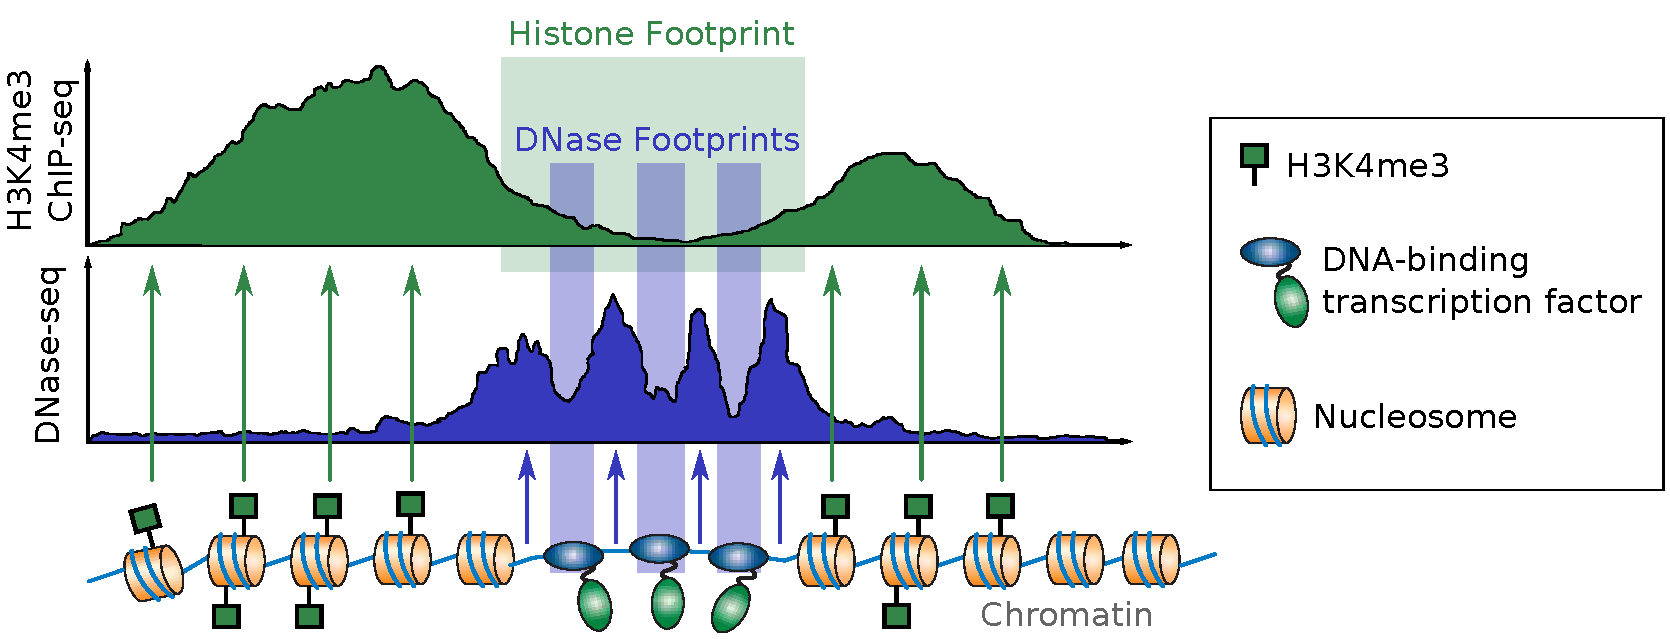
\includegraphics[width=0.75\textwidth]{gusmao_grammar_tfbs}
\caption[Grammar of transcription factor binding sites]{\textbf{Grammar of transcription factor binding sites.} In this figure we show examples of histone modification ChIP-seq and DNase-seq signals for a genomic region (top) and a graphical representation of the chromatin landscape within this region (bottom). We and others observed that there is a clear pattern regarding these signals and the TFBSs. TFBSs happen at depletions between two peaks of the DNase-seq signal. Furthermore, these DNase-seq peaks, which determines an open chromatin region, happen at the depletion between two peaks of active histone modification marks. These putative depletion regions within these peak-dip-peak patterns are termed ``footprints''.}
\label{fig:gusmao_grammar_tfbs}
\end{figure}

%%%%%%%%%%%%%%%%%%%%%%%%%%%%%%%%%%%%%%%%%%%%%%%%%%%%%%%%%%%%%%%%%%%%%
% Section: Types of Computational Footprinting Methods
%%%%%%%%%%%%%%%%%%%%%%%%%%%%%%%%%%%%%%%%%%%%%%%%%%%%%%%%%%%%%%%%%%%%%
\subsection{Types of Computational Footprinting Methods}
\label{sec:types.computational.footprinting.methods}

% Segmentation vs site-centric methods
Computational footprinting methods can be broadly categorized as: (1) segmentation methods and (2) site-centric methods. The main difference between these two groups of computational footprinting methods is the usage of \emph{a priori} predictions of TFBSs based on DNA sequence affinity, i.e. MPBSs (see Section~\ref{sec:motif.matching}).

% Segmentation methods
The rationale behind segmentation methods is to use NGS-based data to scan the genome for footprints. This approach generates a map of putative active binding sites without actually specifying the transcription factors that are binding these regions. The disadvantage is that further processing is necessary in order to identify such transcription factors. However, the advantage of such approach is that novel transcription factors or binding types can be detected.

% Site-centric methods
The rationale behind site-centric methods is that the analysis starts with putative binding sites obtained by using, for instance, a sequence-based prediction method such as motif matching (Section~\ref{sec:motif.matching}). Then, experimental evidence around these \emph{a priori} predictions are gathered and classified using machine learning methods in a supervised or unsupervised fashion. This approach leads to footprints for target TFs. The advantage of such approach is that we already know which TFs are binding to the correctly classified footprints. However, the disadvantage is that it depends on this \emph{a priori} TF evidence, which is not always available. Furthermore, \emph{de novo} motif finding is virtually impossible on footprint predictions obtained with site-centric methods, while it is easily performed on the footprint predictions of segmentation approaches. The Figure~\ref{fig:gusmao_segmentation_vs_sitecentric} provides a graphical representation of the segmentation and site-centric approaches.

% Figure - Segmentation versus site-centric computational footprinting methods
\begin{figure}[h!]
\centering
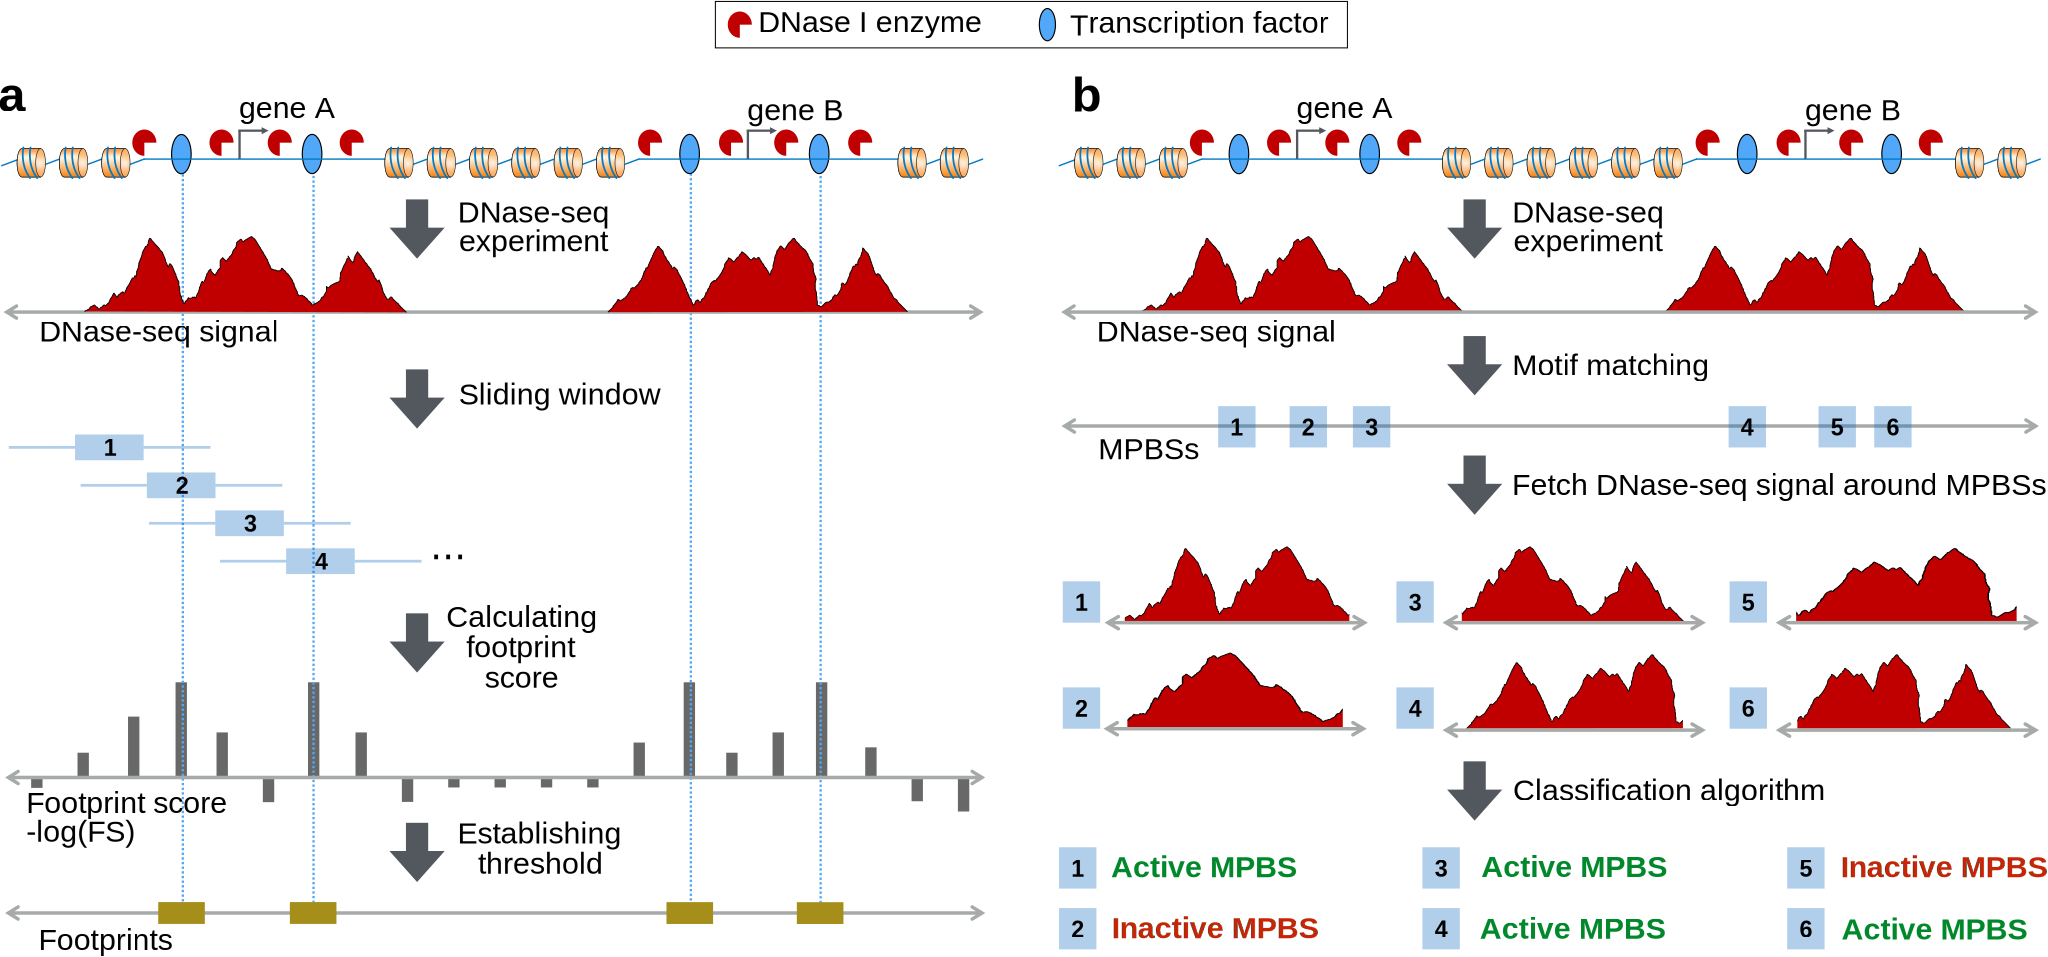
\includegraphics[width=0.99\textwidth]{gusmao_segmentation_vs_sitecentric}
\caption[Segmentation \emph{versus} site-centric computational footprinting methods]{\textbf{Segmentation \emph{versus} site-centric computational footprinting methods.} This figure show an example of each computational footprinting approach using DNase-seq data. Both methods tries to detect the grammar of TFBSs described in Section~\ref{sec:grammar.tfbs}. (\textbf{a}) Graphical representation of the segmentation computational footprinting approach. In this case, the DNase-seq signal is generated by: mapping the DNase-seq reads to the reference genome and counting the overlap of $5\prime$ positions of the reads (see Section~\ref{sec:dnase.seq}). Then, the segmentation approach ``reads'' such signal as a time-series and tries to detect the footprint positions. The output of this method are the genomic regions recognized as footprints given the grammar of TFBSs. (\textbf{b}) The site-centric approach starts by detecting MPBSs using sequence-based algorithms such as motif matching (Section~\ref{sec:motif.matching}). Then, the DNase-seq signal (generated in the same way as in the segmentation approach) around all MPBSs is fetched and submit to a classification method. Such classification method will distinguish the MPBSs that match the grammar of TFBSs (true MPBSs) from the ones that do not (false MPBSs). In this case, the true MPBSs represent the footprint predictions.}
\label{fig:gusmao_segmentation_vs_sitecentric}
\end{figure}

%%%%%%%%%%%%%%%%%%%%%%%%%%%%%%%%%%%%%%%%%%%%%%%%%%%%%%%%%%%%%%%%%%%%%
% Section: Literature Review
%%%%%%%%%%%%%%%%%%%%%%%%%%%%%%%%%%%%%%%%%%%%%%%%%%%%%%%%%%%%%%%%%%%%%
\subsection{Literature Review}
\label{sec:literature.review}

% Introduction
Previously, we discussed that the traditional computational method to identify putative binding sites -- motif matching -- which was devised in order to be able to identify binding sites in a genome-wide manner, is not able to identify active binding sites, since it is only based on the DNA sequence. However, improvements on NGS techniques allowed the adaptation of low-throughput assays in order for them to be able to be applied genome-wide. Nevertheless, the magnitude and complexity of data generated by these novel NGS-based assays such as DNase-seq and ChIP-seq need the aid of computational approaches to make sense of such data. The novel biological experimental methods coupled with state-of-the-art computational approaches led to significant advances in the research of gene regulation and the understanding of the regulatory processes leading to devious phenotypic manifestations, such as diseases. In this section we present a review on state-of-the-art computational footprinting methods.

% Hesselberth (hesselberth2009) - method (Hesselberth)
One of the first attempts to create a computational footprinting method for DNase-seq data was performed by Hesselberth et al.~\cite{hesselberth2009}. In their study, they performed the DNase-seq experiment in the \emph{Saccharomyces cerevisiae} organism (yeast). In possession of such data, they observed that the DNase I enzyme presented a cleavage preference towards some DNA dinucleotide than others. They hypothesized that such issue, which they termed ``sequence-based biases in DNase I cleavage'', might lead to biased results, since there would be a higher concentration of DNase-seq signal at particular genomic regions than others. Therefore, in order to correct for such sequence-based cleavage bias they analyzed $3.27$ million cleavage positions from naked \emph{Saccharomyces cerevisiae} DNA. Their correction strategy consisted in using dinucleotide cleavage frequencies in naked DNA \emph{versus} genomic dinucleotide frequencies in order to correct the genomic signal from the original DNase-seq experiment. In posession of the corrected DNase-seq signal, they used a three-phase segmentation approach to detect footprints in the DNase-seq data. In the first phase, they considered every possible window $k = [k_{min},k_{max}]$ that was contained within one of the specified target regions (DHSs) and computed a depletion score for each of these regions. In the second phase, they selected high-scoring windows using a greedy algorithm, eliminating from consideration any window that overlapped a window with a higher score. Finally, in a third phase, they shuffled the input data independently within each target region and repeated the entire procedure, using the resulting scores to estimate $q$-values. They introduced the ``footprint score'' (FS) as a depletion score. The FS is defined as the ratio between the amount of DNase I cleavage within the footprint and the amount of DNase I cleavage in the footprint's flanking regions. More formally, let the interval ${k} = [{m},{n}]$ be a putative footprint region and $\mathbf{x} = \langle  x_1, ..., x_G\rangle$ be the DNase-seq genomic signal from a genome of size $G$. The FS can be calculated as 
\begin{equation}
  \label{eq:fs1}
  \text{FS}_{k} = -\left(\frac{{n}_{C}+1}{{n}_{R}+1} + \frac{{n}_{C}+1}{{n}_{L}+1}\right),
\end{equation}
where
\begin{align}
  \label{eq:fs2}
  {n}_{C} &= \sum_{j=m}^{n} {x}_{j}, &
  {n}_{R} &= \sum_{j=n}^{2n-m} {x}_{j}, &
  {n}_{L} &= \sum_{j=2m-n}^{m} {x}_{j}.
\end{align}

% Hesselberth (hesselberth2009) - results
Within this systematic identification of DNase I footprints, Hesselberth et al.~\cite{hesselberth2009} analyzed many features regarding such computational footprinting. They identified many known sequence motifs in these footprints, observing that collectively, $35.2\%$ of the footprints with a false discovery rate of $0.05$ overlapped a conserved factor binding site inferred from ChIP data. Furthermore, they observed that the patterns of DNase I protection surrounding different TFs had different average shapes, i.e. the DNase-seq average signal varies depending on the binding type of TFs. Finally, they created a very consistent genome-wide map of transcription factor binding sites for the \emph{Saccharomyces cerevisiae}, which led into insights on the chromatin architecture and gene expression of this organism.

% Whitington (whitington2009) / Won (won2010)
Two other computational footprinting methods by Whitington et al.~\cite{whitington2009} and Won et al.~\cite{won2010} used ChIP-seq for histone modifications in order to assess TFBS footprints. In Whitington et al.~\cite{whitington2009} they used data regarding histone modification H3K4me3 to infer TFBSs for 14 mouse TFs and 10 human TFs. They used a site-centric approach that consists on simple filters for MPBSs. These filters consist on regarding a MPBS as true if the density of H3K4me3 was above certain \emph{ad hoc} thresholds. They showed that using histone modification H3K4me3 information to filter out false positive MPBSs significantly improves the accuracy in comparison to the unfiltered MPBSs alone. Furthermore, they showed that H3K4me3 filters outperformed other filters based on proximity to transcription start sites (TSSs) or phylogenetic conservation. Won et al.~\cite{won2010} used a more complex approach -- termed Chromia -- which detects footprints with HMMs in a site-centric manner. Chromia uses a multivariate HMM which integrates continuous H3K4me3 signals and PWM scores. Their HMM models have three components, which are trained separately: (1) a promoter-proximal component -- trained around TSS regions with strong h3K4me3; (2) a distal enhancer component -- trained around p300 binding sites with strong H3K4me2 and H3K4me3 signals and (3) background -- trained in the whole chromosome 1. The authors showed that Chromia significantly outperformed competing approaches in a gold standard TFBS set created using 13 TFs binding evidence (ChIP-seq and RNA interference knockdown) binding in mouse embryoinic stem cells.

% Peak-dip-peak
Both Hesselberth et al.~\cite{hesselberth2009} and Won et al.~\cite{won2010} explored the peak-dip-peak pattern within DNase-seq and histone modification ChIP-seq data, respectively. These authors observed that there is a clear TFBS grammar related to DNase-seq and histone modifications. This grammar, depicted in Figure~\ref{fig:gusmao_grammar_tfbs}, shows that TFBSs happen at depletions between two peaks of the DNase-seq signal, which is located within DHs which occur whithin a depletion between two peaks of activating histone marks.

% Neph (neph2012a)
Neph et al.\cite{neph2012a} used a simplified version of the segmentation-based method originally proposed in~\cite{hesselberth2009}. Their method consists on applying a sliding window to find genomic regions ($6$--$40$ bp) with low DNase-seq signal between regions ($3$--$10$ bp) with high DNase-seq signal (peak-dip-peak pattern). They performed their experiments on human DNase-seq data generated using the double-hit protocol. They also evaluate the footprint score (FS) to determine the most significant predictions. Their study amplified the analysis scale significantly, by detecting footprints for $41$ diverse human cells with data from the ENCODE repository~\cite{encode2012}. Such a large-scale study was able to provide multiple new insights on computational footprinting. First, they found that genetic variants affecting allelic chromatin states are concentrated in footprints, and that these elements are preferentially sheltered from DNA methylation. Second, they showed that the average TF-wise patterns of DNase I digestion can be correlated to the crystallographic topography of protein-DNA interfaces, indicating that TF structure has been evolutionarily imprinted on the genome. Finally, they performed an extensive ``brute force'' \emph{de novo} motif finding algorithm and found $683$ unique motif structures, of which $394$ ($58\%$) matched distinct experimentally-verified motif models present in Jaspar~\cite{mathelier2014}, Uniprobe~\cite{robasky2011} and Transfac~\cite{matys2006} motif repositories.

% Boyle (boyle2011)
Boyle et al.~\cite{boyle2011} designed a segmentation computational footprinting approach, which is based on using hidden Markov models (HMMs) to predict the DNase-seq pattern described in Figure~\ref{fig:gusmao_grammar_tfbs}. They performed their experiments on human DNase-seq data generated using the single-hit protocol. Briefly, their HMM uses a normalized DNase-seq cleavage signal to find regions with depleted DNase I digestion (footprints) between two peaks of intense DNase I cleavage. As the DNase-seq profiles required a nucleotide-resolution signal, which is usually noisy, the authors used a Savitzky-Golay smoothing filter to reduce noise and to estimate the slope of the DNase-seq signal~\cite{madden1978}. Their HMM had five states, with specific states to identify the decrease/increase of DHS signals around the peak-dip-peak region. They also provided numerous insights into computational footprinting. First, they described cell-specific footprint patterns, which correlates significantly with gene expression fold change between different cells. Second, they described a conservation phenomenon which was not observed in the conservation study performed by Hesselberth et al.~\cite{hesselberth2009}. They find that for most TFs, there is a marked drop in conservation \approxy$10$ bp immediately flanking the footprint. Beyond this drop, conservation increases again before gradually decreasing to background levels, creating a ``shoulder'' in this signal. They also described in details the unique binding characteristics that the human insulator CTCF footprints displays. Finally, they used the STAMP~\cite{mahony2007} method to detect putative TFs in footprints, which simply searches for TFs on known DNA sequence affinity information. Therefore, a \emph{de novo} motif finding approach was not performed as in Neph et al.\cite{neph2012a}.

% Pique-Regi (pique2011) (Centipede) 
Nevertheless, one of the most used footprinting approaches was created by Pique-Regi et al.~\cite{pique2011}. Their stratey, termed Centipede, is a site-centric approach, which gathers experimental and genomic information around motif-predicted binding sites (MPBSs). It then uses a Bayesian mixture model as an unsupervised classification tool to label each retrieved MPBS as either `bound' or `unbound'. Their approach was the first to integrate multiple different experimental assays. The experimental includes DNase-seq and histone modification ChIP-seq. The DNase-seq data was used at the nucleotide-resolution, by fetching raw DNase-seq signal surrounding a $200$ bp window around each MPBS. However, only the average histone modification ChIP-seq signal was used. The genomic data used includes PWM bit-score, sequence conservation and distance to the nearest TSS. They evaluated their approach on six TFs with ChIP-seq data available. Their gold standard was created as follows. First, they overlapped the MPBSs with TF ChIP-seq peaks. If a MPBS overlapped with a ChIP-seq peak, it was considered a ``true MPBS''; otherwise, it was considered a ``false MPBS''. Then, they were able to quantify the amount of true positive, false positive, true negative and false negative predictions by overlapping their footprints with the true/false MPBS gold standard (see Section~\ref{sec:chipseq.evaluation}). With such gold standard they were able to calculate receiver operating characteristic (ROC) curves and evalute the area under the ROC curve (AUC). Their reported average AUC for the six tested TFs were as high as $98.11\%$. However, they did not observe a gain in accuracy when using a model with both DNase-seq and histone modification ChIP-seq (median AUC $= 96.52\%$). Furthermore, although their method is site-centric they were able to devise a \emph{de novo} motif finding algorithm. However this algorithm is time consuming and relies on the usage of \emph{a priori} information of genomic $k$-mer distributions.

% Cuellar (cuellar2012)
Cuellar-Partida et al.~\cite{cuellar2012} proposed a site-centric method to include NGS-based experimental data as priors for the motif matching procedure (see Section~\ref{sec:motif.matching}). Their method uses a probabilistic classification approach inspired in Bayes decision theory to compute better log-posterior odds scores than the ones observed by purely using the PWM structure. Before the computation of prior probabilities the DNase-seq or histone modification ChIP-seq signals are smoothed as follows. To create smoothed DNase-seq signals they evaluated the number of reads aligning to a window of $150$ bp, specified every $20$ bp. Histone modification smoothed signal input data was specified in a $25$ bp resolution. In every position, it was summed $ 1 $ if a mapped read fell within $0$--$200$ bp from the $25$ bp window and $ 0.25 $ if it occurred within $200$--$300$ bp. After the computation of prior probabilities with smoothed DNase-seq signal, they perform the motif match using the program FIMO~\cite{grant2011}. They performed the first comparative study on computational footprinting methods, where they compared their method with Centipede and with a much simpler approach termed here as ``tag count'' (TC). This site-centric approach corresponds to the number of DNase I cleavage hits within a window of length $L$ around a certain genomic interval (in this case, MPBSs). More formally, let the interval ${k} = [{m},{n}]$ be a putative MPBS region and $\mathbf{x} = \langle x_1, ..., x_G\rangle$ be the DNase-seq genomic signal from a genome of size $G$. The TC can be calculated as 
\begin{equation}
  \label{eq:tc}
  \text{TC}_{k} = \sum_{j={\frac{m+n}{2}-\frac{L}{2}}}^{\frac{m+n}{2}+\frac{L}{2}-1} {x}_{j}.
\end{equation}
Their results showed that, for their approach, the DNase-seq method dramatically improved the sequence-based prediction of TFBSs. Furthermore, they find that adding the histone modifications H3K4me3 or H3K27ac to their DNase-seq model improved the accuracy slightly. The comparison showed that Centipede outperformed their method using the gold standard proposed in Pique-Regi et al.~\cite{pique2011}. However, in this case, they found that using the simple TC approach would outperform both Centipede and their approach. They associate such results with the biases generated by such MPBS-centric gold standard.

% Piper (piper2013) (Wellington)
Piper et al.~\cite{piper2013} devised a segmentation approach based on a Binomial test. For a given candidate footprint, it tests the hypothesis that there are more reads in the flanking regions than within the footprint. Following an observation that DNase-seq cuts of the double-hit protocol are strand-specific, Wellington only considers reads mapped to the upstream flanking region of the footprints. They evaluate their method and competing methods in a gold standard created with 214 human TF ChIP-seq data sets. First, they showed that using such observed strand imbalance of reads increases the computational footprinting predictive power. Furthermore, their strategy outperformed competing methods Hesselberth et al.~\cite{hesselberth2009}, Neph et al.~\cite{neph2012a} and Centipede~\cite{pique2011}. Finally, a great contribution on this paper is the creation of a DNase-seq data processing package in the programming language Python termed pyDNase. Such package allows a user-friendly application of their methodology and also further DNase-seq data processing tools.

% Sherwood (sherwood2014) (PIQ)
Sherwood et al.~\cite{sherwood2014} developed a computational footprinting framework termed protein interaction quantification (PIQ). PIQ is a site-centric method, which uses Gaussian process to model and smooth the footprint profiles around candidate MPBSs ($100$ bp up/downstream)~\cite{sherwood2014}. Active footprints are estimated with an expectation propagation algorithm. Finally, PIQ indicates the set of motifs which footprint signals are distinguishable from noise to reduce the set of candidate TFs. They compared their method with competing methods in a very large benchmarking data set containing $303$ TFs binding on K562 human cell line. Through the same evaluation procedure used in the aforementioned works~\cite{pique2011,cuellar2012,piper2013}, they measured a mean AUC of $0.93$ for PIQ against $0.87$ for Centipede~\cite{pique2011} and $0.65$ for Neph et al.~\cite{neph2012a} approach. Nevertheless, this study contains many side analyses which provided insights into computational footprinting. They analyzed the differentiation of mouse embryonic stem cells into prepancreatic and intestinal endoderm cells and were able to identify and experimentally validate eight pioneer TF families that perform changes in the chromatin dynamics. One of the most interesting findings is that these pioneer TFs change the chromatin in a directional manner. Besides the identification of pioneer TFs, they also detected ``settler'' TFs, which binds the DNA after the chromatin structure changes performed by the pioneer TFs.

% He et al (he2014)
At this point, He et al.~\cite{he2014} revived the discussion proposed by Cuellar-Partida et al.~\cite{cuellar2012} on the feasibility of computational footprinting methods and the comparison of their performance \emph{versus} simple metrics for ranking footprints (such as the TC). They showed that the FS scoring metric proposed in Hesselberth et al.~\cite{hesselberth2009} and used by Neph et al.~\cite{neph2012a} is heavily impacted by the DNase-seq cleavage bias in comparison to the simpler TC ranking strategy. They also showed that some TFs, such as nuclear receptors, does not present a clear peak-dip-peak pattern as shown in Figure~\ref{fig:gusmao_grammar_tfbs}. Instead, these TFs contain an average DNase-seq pattern that resembles the DNase I sequence cleavage bias evaluated on naked DNA DNase-seq.

% Yardimci (yardimci2014) (FLR)
The issues on computational footprinting presented by He et al.~\cite{he2014} were addressed in Yard{\i}mc{\i} et al.\cite{yardimci2014}. In this study, they proposed a site-centric method based on a mixture of multinomial models to detect classify MPBSs as active/inactive in an unsupervised manner. The method uses an expectation maximization algorithm to find a mixture of two multinomial distributions, representing active (footprints) and inactive (background) MPBSs. The background model is initialized with either cleavage bias frequencies or estimated {\emph de novo}. After successful estimation, MPBSs are scored with the log odds ratio for the footprint \emph{versus} background model. The model takes DNase-seq cuts within a small window around the candidate profiles ($25$ bp up/downstream) as input. DNase-seq cleavage bias is estimated for 6-mers based on the DNA sequences extracted within the same regions in which the cuts were retrieved. They showed that their method significantly outperformed the simple TC approach. Furthermore, they also criticise the TF ChIP-seq evaluation method on the basis that it is not able to identify indirect binding events. For that reason, they performed a simple analysis based on gene expression and were able to observe that the footprints retrieved by their approach were significantly enriched on cell types where the tested TFs were being expressed.

% Sung (sung2014) (DNase2TF)
Sung et al.~\cite{sung2014} also performed a number of analysis that contributed to the discussion initiated in He et al.~\cite{he2014}. First, they developed a new segmentation computational footprinting approach with very simple premisses, which was called DNase2TF. DNase2TF is based on a binomial $z$-score, which evaluates the depletion of DNase-seq reads around the candidate footprints. At a second step, DNase2TF interactively merges close candidate footprints whenever they improve depletion scores. DNase2TF corrects for DNase I cleavage bias using cleavage statistics for $2$ or $4$-mers. They reported that their method outperformed Hesselberth et al.~\cite{hesselberth2009}, Centipede~\cite{pique2011} and Wellington~\cite{piper2013}. Their evaluation data set used only ChIP-seq information without MPBSs, leading to ROC-like curves in which the curves could stop in the middle of the sensitivity \emph{versus} specificity spectrum given the lack of negative samples. Although their evaluation is hard to compare to previous approaches, they also raised the issue seen by He et al.~\cite{he2014} that some TF DNase-seq signature ressembles their cleavage bias. Furthermore, they showed that one of the main problems with DNase I footprinting was related to the fact that some TFs have a very low residence time on DNA. Since they bind to the DNA in a short time period, the DNase-seq protocol is not able to produce a clear peak-dip-peak pattern.

% Kahara (kahara2015) (BinDNase)
Finally, K\"{a}h\"{a}r\"{a} et al.~\cite{kahara2015} developed a supervised site-centric method based on logistic regression to predict active/inactive MBBSs. The algorithm starts with base pair resolution DNase-seq signal around the MPBSs ($100$ bps up/downstream) and selects discriminatory features using a backward greedy approach. As a supervised approach, the method requires positive and negative examples, which can be obtained from TF ChIP-seq data. They showed that their approach does not present any significant gain in performance by modelling DNase-seq cleavage bias. Furthermore, they present a discussion on the standardization of DNase-seq data preprocessing, showing that data on major repositories such as ENCODE are not always analyzed in a standard manner. They state that their supervised approach outperforms unsupervised site-centric approaches such as Centipede~\cite{pique2011} and PIQ~\cite{sherwood2014}. However, they acknowledge the fact that their approach can only be executed when TF binding evidence (such as TF ChIP-seq) is available \emph{a priori} for model training.

% Conclusion
All methods described here presented a different approach to address the problem of active binding site detection. They used different gold standards and point out different biases related to the usage of NGS-based techniques. Furthermore, each study performs a method comparison using a different set of competing methods, which does not seem to encompass all the diversity of methods in the literature. A summary of these methods and their features is presented in Table~\ref{tab:overview_methods}.

% Table -  Overview of methods
\begin{footnotesize}
\begin{longtable}{p{1.4cm}p{0.6cm}p{1.7cm}p{1.3cm}p{1.6cm}p{1.6cm}p{0.8cm}p{0.8cm}p{2cm}}
\caption[Overview of methods]{\textbf{Overview of methods.} We list here the main characteristics of the evaluated methods. Methods are characterized by their type (SC -- site centric \emph{versus} SEG -- segmentation approach), algorithm, bias correction strategy, resolution/smoothing strategy, method for ranking footprints, availability and usability. Concerning availability, methods obtain a `+' if they are public available (`--' otherwise). Boyle method is not public, but authors provide footprint predictions of a few cells. The code for Neph was obtained upon request to authors. Concerning usability, methods natively supporting standard genomic files and being executed with few commands ($\leq3$) have `+' (`--' otherwise).} \\
\label{tab:overview_methods} \\
  \hline
    Name & Type & Algorithm & Bias Correction & Resolution Smoothing & Footprint Ranking & Availa- bility & Usa- bility & Others\\
  \hline
    BinDNase & SC & Logistic Regression & No & bp / Sliding Window & Probability & + & -- & Require TF ChIP-seq for Training\\
    Boyle & SEG & HMM & No & bp & None & -- & -- & \\
    Centipede & SC & Bayesian Mix. Model & No & bp & Probability & + & -- & Integrates Histone and Sequence Data\\
    Cuellar & SC & Weighted Motif Match & no & Sliding Window & PWM Score & + & -- & \\
    DNase2TF & SEG & Sliding Window & 4-mer & bp & $p$-values & + & + & \\
    FLR & SC & Mixture Model & 6-mer & bp & Log-Odds & + & -- & Bias Correction for Each TF\\
    HINT-BC & SEG & HMM & 6-mer & bp & TC & + & + & Integrates Histones\\
    Neph & SEG & Sliding Window & no & bs & FS & -- & -- & \\
    PIQ & SEG & GP/Expectation Propagation & No & bp / GP & Probability & + & + & Support Replicates, Time Series\\
    Wellington & SEG & Sliding Window & No & bp & $p$-value & + & + & \\
  \hline
\end{longtable}
\end{footnotesize}

%%%%%%%%%%%%%%%%%%%%%%%%%%%%%%%%%%%%%%%%%%%%%%%%%%%%%%%%%%%%%%%%%%%%%
% Subsection: Current Challenges
%%%%%%%%%%%%%%%%%%%%%%%%%%%%%%%%%%%%%%%%%%%%%%%%%%%%%%%%%%%%%%%%%%%%%
\subsection{Current Challenges}
\label{sec:current.challenges}

% Introduction
As seen in Section~\ref{sec:literature.review} a number of computational footprinting methods have been proposed. However, there are still many challenges not addressed by these methods. In this section we will discuss the current challenges on computational footprinting methods.

% Signal treatment
It is known that NGS-based genomic signals are very noisy and intrinsically complex. Most methods used some sort of smoothing approach to handle such complexity~\cite{pique2011,cuellar2012,sherwood2014,kahara2015}. Although a few attempts have been made to use these signals in their maximum possible resolution~\cite{boyle2011,sung2014}, not much attention was given to the proper mathematical modelling of these complex signals. The NGS-based genomic signals can be affected by multiple artifacts stemming from either the biological protocol or the computational pre-processing steps, such as: (1) chromatin fragmentation and size selection, (2) tissue-specific signal variability generated by the phenol chloroform extraction step commonly used to separate nucleic acids from protein, (3) PCR amplification biases and duplications, (4) particularities of read mapping algorithms and (5) TF binding characteristics. These artifacts were summarized recently by Meyer et al.~\cite{meyer2014}.

% Integrative approaches
Furthermore, none of the computational footprinting methods so far took full advantage of the nucleotide-resolution signal generated for DNase-seq and histone modifications ChIP-seq signal. The current integrative approaches usually takes only the nucleotide-resolution signal for one of the signals, such as DNase-seq in the Centipede~\cite{pique2011} method. The main reason discussed by most integrative approaches~\cite{pique2011,cuellar2012} is that it is hard to integrate signals which has a high degree of variation.

% Evaluation
Moreover, there is no well-defined gold standard for the evaluation of footprinting methods. All work so far has used ChIP-seq of TFs in conjunction with motif-based predictions (MPBSs) as ground truth. In short, MPBSs supported by ChIP-seq peaks are positive examples (true TFBSs), while MPBSs without ChIP-seq support are negative examples (false TFBSs)~\cite{cuellar2012}. This evaluation requires TF ChIP-seq experiments to be carried out on the very same cells as the DNase-seq experiment and has a few caveats. First, TF ChIP-seq peaks are also observed in indirect binding events~\cite{yardimci2014}. Second, they have a lower spatial resolution than DNase-seq. Therefore, false TFBSs might be regarded as true TFBSs by proximity to a real TFBS of a distinct TF~\cite{cuellar2012,yardimci2014}.

% Bias-correction
As previously mentioned, He et al.~\cite{he2014} showed that sequence cleavage bias around TFBSs strongly affects the performance of a computational footprinting method (FS) in a TF-specific manner. Such impact is depicted in Figure~\ref{fig:he_cleavage_bias}. They also indicated several TFs, such as nuclear receptors and \emph{de novo} motifs found via computational footprinting~\cite{neph2012a}, where the DNase-seq profile resembles their sequence cleavage bias estimate. Furthermore, they indicated that ranking putative TFBS by the number of DNase-seq reads around putative TFBSs (TC) outperforms the ranking by FS, which is used by some computational footprinting methods~\cite{hesselberth2009,neph2012a}.

% Figure - Impact of DNase I cleavage bias on computational footprinting
\begin{figure}[h!]
\centering
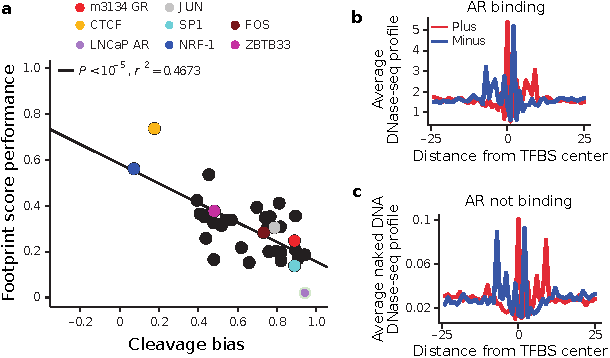
\includegraphics[width=0.45\textwidth]{he_5_cleavage_bias}
\caption[Impact of DNase I cleavage bias on computational footprinting]{\textbf{Impact of DNase I cleavage bias on computational footprinting.} This graph shows the amount of sequence cleavage bias ($x$-axis) \emph{versus} the performance of the FS footprinting method. We can clearly observe that there is a strong negative correlation between these two variables. \emph{Source: He et al.}\cite{he2014} (modified to fit thesis format and/or clarify key points).}
\label{fig:he_cleavage_bias}
\end{figure}

% TF residence time
Besides the sequence cleavage bias, another experimental aspect affecting the computational analysis of DNase-seq is the residence time of TF binding. Sung et al.~\cite{sung2014} showed that short-lived TFs display a lower DNase I cleavage protection pattern, i.e. low number of DNase-seq reads surrounding the footprint (see Figure~\ref{fig:sung_residence_time}). Such fleeting transcription factors would not be detectable by methods that search for such protection pattern on DNase-seq data.

% Figure - Transcription factor residence time
\begin{figure}[h!]
\centering
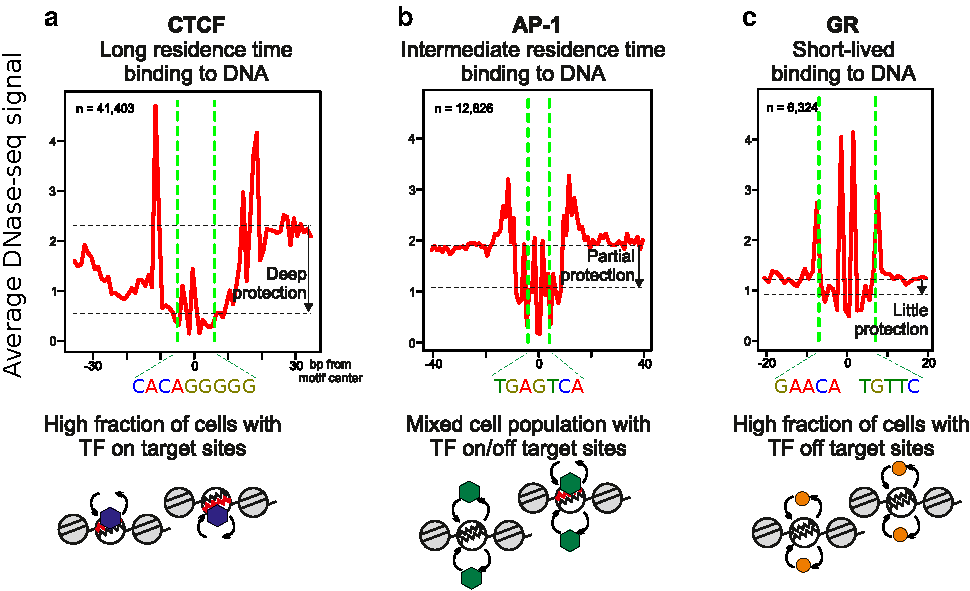
\includegraphics[width=0.8\textwidth]{sung_9_residence_time}
\caption[Transcription factor residence time]{\textbf{Transcription factor residence time.} This graphs depicts the average DNase-seq signal around TFBSs of transcription factors with: (a) long residence time -- CTCF; (b) intermediate residence time -- AP-1 (C-jun) and (c) short residence time -- GR. Sung et al.~\cite{sung2014} discuss that the width of the protection against the DNase I enzyme might be correlated with the residence time of the transcription factors in the DNA. \emph{Source: Sung et al.}\cite{sung2014} (modified to fit thesis format and/or clarify key points).}
\label{fig:sung_residence_time}
\end{figure}

% Disagreement on aplicability of computational footprinting
As a matter of fact, there has been a discussion in the literature regarding the applicability of computational footprinting methods \emph{versus} more simple approaches~\cite{he2014,meyer2014}. According to He et al.~\cite{he2014} and Cuellar-Partida et al.~\cite{cuellar2012}, the simple statistic to rank MPBSs -- tag count (TC) -- can be applied instead of more complex methods. Such discussion led to some disagreement on the literature on whether computational footprint methods were really useful. In this work we will analyze all these claims in detail.

%%%%%%%%%%%%%%%%%%%%%%%%%%%%%%%%%%%%%%%%%%%%%%%%%%%%%%%%%%%%%%%%%%%%%
% Subsection: Addressing the Computational Footprinting Problem
%%%%%%%%%%%%%%%%%%%%%%%%%%%%%%%%%%%%%%%%%%%%%%%%%%%%%%%%%%%%%%%%%%%%%
\subsection{Addressing the Computational Footprinting Problem}
\label{sec:addressing.computational.footprinting}

% Introduction
The current challenges described in Section~\ref{sec:current.challenges} motivated our analysis on computational footprinting methods. We observed that there are multiple open research oportunities within this area and many features which were not explored by previous methods.

% Better signal treatment
Regarding the signal treatment, current methodologies have used only standard normalization approaches. Our analysis will focus on finding an approach to assuage the variabilities within a dataset (generated by PCR amplification, particularities of read mapping algorithms and TF binding characteristics) and between different datasets (generated by protocol technicalities, such as the separation of DNA from protein in the extraction steps). We also plan to perform empirical analyses on different types of signal treatment.

% Cleavage bias correction
Furthermore, although a number of methods have tried to correct for sequence cleavage bias~\cite{hesselberth2009,yardimci2014,sung2014}, a more comprehensive study is necessary. First, a detailed picture on the nature of such bias is needed. Second, estimation methods have to be formalized. Third, the correction strategies have to be tested agains uncorrected methods in order to assess the importance of such correction. Nevertheless, only a very simple method (FS) was tested and observed to be affected by sequence cleavage bias. Such test needs to be extended for more robust computational footprinting methods. Moreover, other experimental artifacts might also have an impact on the footprinting method's performance. We will analyze all these issues.

% Integrative multivariate hidden markov model and eletronic filters
The main contribution of this work is the development of novel computational footprinting methods. We will use two different approaches for the problem and observe their behaviour. The first approach will use the state-of-the-art computational segmentation method multivariate continuous hidden Markov models. The second approach will use a simplified approach based on eletronic filters. The rationale is that we will tackle the problem with a more robust computational approach and then verify if simpler methodologies can be used instead, as proposed by He et al.~\cite{he2014}. Moreover, as previously mentioned, there are no existing computational footprinting method so far that has taken full advantage of nucleotide-level resolution of DNase-seq signals in combination with histone modification ChIP-seq signals. Here we will try to integrate these signals and observe the impact on performance.

% Address the problem of residence time
We should also analyze the impact of transcription factor residence time on computational footprinting methods. First, we will assess if this is a problem to be considered, by evaluating the issue in a systematic manner with more transcription factors than in Sung et al.~\cite{sung2014}. Such problem is virtually impossible to be corrected computationally, since is an intrinsic experimental limitation. However, we should try to find some insights that might aid in the detection of problematic transcription factors.

% Make a standardized evaluation benchmark data set
Moreover, we plan to create a standardized benchmarking evaluation data set. Such benchmarking data set will consider all machine learning evaluation best practises in order to reduce biases and enhance reproducibility. Such benchmarking attempt aids in providing transparency and correctness of research.

% Design a ChIP-seq free evaluation approach
As mentioned in Section~\ref{sec:current.challenges}, the traditional evaluation approach, based on transcription factor ChIP-seq, have some intrinsic biases. We will also work on the creation of yet another evaluation scenario which does not involve transcription factor ChIP-seq data. Recently, Yard{\i}mc{\i} et al.\cite{yardimci2014} indicated that footprint quality scores, as measured by the footprint likelihood ratio (FLR), were significantly higher in cells where the TF was expressed. This observation indicates that comparing changes in expression and quality of footprints in a pairs of cells could provide an alternative footprint evaluation measure.

% Comprehensive method comparison
Also, with the exception of a few studies, comparative analyses evaluating footprinting methods were based on ChIP-seq of few ($< 12$) TFs and a maximum of four competing methods were evaluated. Despite the importance of method evaluation, there is a clear lack of studies performing a comprehensive analysis of computational footprinting methods. Here, we will analyze all state-of-the-art computational footprinting methods published in high impact journals. Such comprehensive analysis will consider current machine learning standards which enables the accurate observation of these methods particularities from multiple evaluation points of view.

% Further results
Finally, we should use our computational footprinting framework in order to provide some empirical insights in the comparison of method's performance with genomic features such as: footprint spatial specificity, transcription factor binding particularities, transcription factor families and CG content.

%%%%%%%%%%%%%%%%%%%%%%%%%%%%%%%%%%%%%%%%%%%%%%%%%%%%%%%%%%%%%%%%%%%%%
% Section: Discussion
%%%%%%%%%%%%%%%%%%%%%%%%%%%%%%%%%%%%%%%%%%%%%%%%%%%%%%%%%%%%%%%%%%%%%
\section{Discussion}
\label{sec:discussion.2}

% Conclusion
In this section we presented all the biological and computational background necessary for the understanding of this work. Then we introduced the problem of the prediction of active transcription binding sites and provided a historical view on how such problem was addressed. First, we presented the traditional computational approach, termed motif matching. Such an approach generates many false positives since it is unable to capture cell-specific chromatin dynamics. Then, we presented the state-of-the-art approach which combines NGS-based techniques with computational frameworks, known as computational footprinting methods.


